% arara: lualatex: { shell: yes, action: nonstopmode, synctex: yes}
% arara: lualatex: { shell: yes, action: nonstopmode, synctex: yes}
% asarara: lualatex: { shell: yes, action: nonstopmode, synctex: yes,  options: "-output-directory=_build"}
% asarara: lualatex: { shell: yes, action: nonstopmode, synctex: yes,  options: "-output-directory=_build"}
\documentclass[landscape]{article}
\usepackage[ngerman]{babel}
\usepackage[no-math]{fontspec}

\usepackage{mwe}
\usepackage{luacode}
\usepackage{shellesc}
% \documentclassw[11pt, a4paper,ngerman]{article}
\usepackage{basicff}
\usepackage{sectsty}
\usepackage{adjustbox} % minipage top allign
\usepackage{subfigure} % Bilder nebeneinander darstellen

\usetikzlibrary{patterns} % preamble
\tcbuselibrary{skins} % preamble

\usepackage{tikz}
% \usepackage{PTSansNarrow}
\usetikzlibrary{matrix}

\usepackage{pgfplots}
\pgfplotsset{
 compat=newest
  }
\tcbset{colframe=red!75!black}
\newenvironment{proggen}{\begin{center}}{\end{center}}

\usepackage{array}
% \setmainfont[Path=/Applications/Microsoft Word.app/Contents/Resources/Fonts/]{Calibri.ttf}
% \setsansfont[Path=/Applications/Microsoft Word.app/Contents/Resources/Fonts/]{Calibri.ttf}
% \setmonofont[Path=/Applications/Microsoft Word.app/Contents/Resources/Fonts/]{Calibri.ttf}
% \usepackage{datetime}
% \pagestyle{fancy}


\setmainfont{UbuntuL.ttf}
\setsansfont{UbuntuR.ttf}
\setmonofont{UbuntuMonoR.ttf}

\newcolumntype{C}[1]{>{\centering\arraybackslash}m{#1}}

\oddsidemargin-10mm
\title{
\color{white}
\begin{center}
 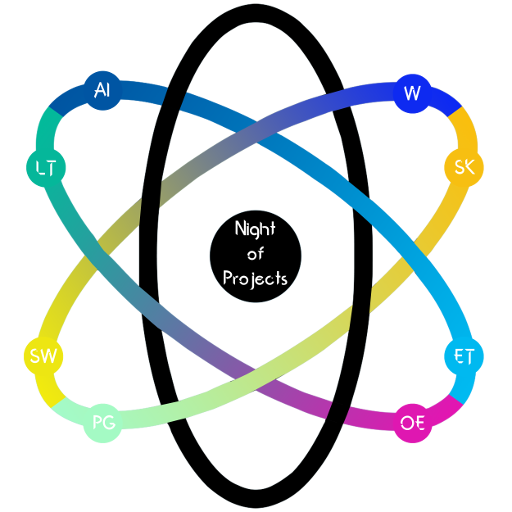
\includegraphics[scale=1.0]{./pictures/NoPLogo.png}
\end{center}
 $\bullet$ \\
 % $\bullet$ \\ $\bullet$ \\
 \color{black}
 % \color{white}
 % $\bullet$ \\
 \color{black}
 Bau eines Delta 3D Druckers from scratch
\color{white}
$\bullet$ \\
\color{black}
%  \begin{center}
% 	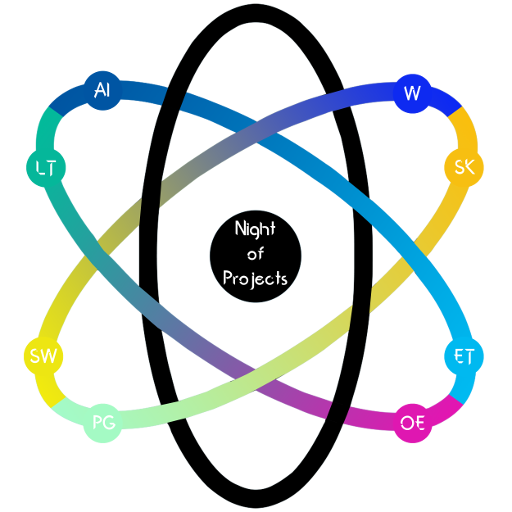
\includegraphics[scale=0.5]{./pictures/NoPLogo.png}
% \end{center}
 % \includegraphics{./pictures/wohnzimmer.png}
}
% \includegraphics{./pictures/asrock.png} Q1900M \\ \color{white} $\bullet$ \\ $\bullet$ \\ $\bullet$ \\ \color{black} \\ \apple \\ 10.10.3

\author{Daniel Krah}
% \rfoot{Compiled on \today\ at \currenttime}
% \cfoot{}
% \lfoot{Page \thepage}
% \date{1.6.2015}

\begin{document}
\huge


\sectionfont{\Huge}
\subsectionfont{\Huge}
\subsubsectionfont{\Huge}
\paragraphfont{\Huge}


\AddToShipoutPicture{\BackgroundPic}
\maketitle%
\newpage%
 % \tableofcontents%
% \newpage
%==================================================================================
% \begin{center}
% \textbf{Vorwort}
% \end{center}



%
% \input{hardware.tex}







%  To Do
% \input{todo.tex}
% \newpage
% \section{Überblick}


% \begin{displaymath}
%   E = \frac{m_{0} c^{2}}{\sqrt{1-v^{2}/c^{2}}}
% \end{displaymath}

% \begin{luacode}
%   for x=1,600 do
%     tex.print(x+2)
%   end
% \end{luacode}
\section{Bauformen von 3D Druckern}
Welche Arten von 3D Druckern gibt es ?
\subsection{Drucker nach Materialart}
\begin{itemize}
  \item \textbf{\uuline{SLA - Drucker}}
  \subitem \textbf{Stereolithografie}
  \subitem Erfinder: 1983  Chuck Hull
  \subitem Ebenfalls: STL-Schnittstelle
  \subitem (STereoLithography, Standard Tessellation Language)
  \item \textbf{\uuline{FDM - Drucker}}
  \subitem \textbf{Fused Deposition Modeling}
  \subitem 1985+ S. Scott Crump
  \subitem Auf Deutsch Schmelzschichtung
  \subitem Fused Filament Fabrication (FFF)
\end{itemize}


\newpage


\subsubsection{SLA - Stereolithografie - Drucker}

\begin{center}
  \vspace{-0.5cm}
  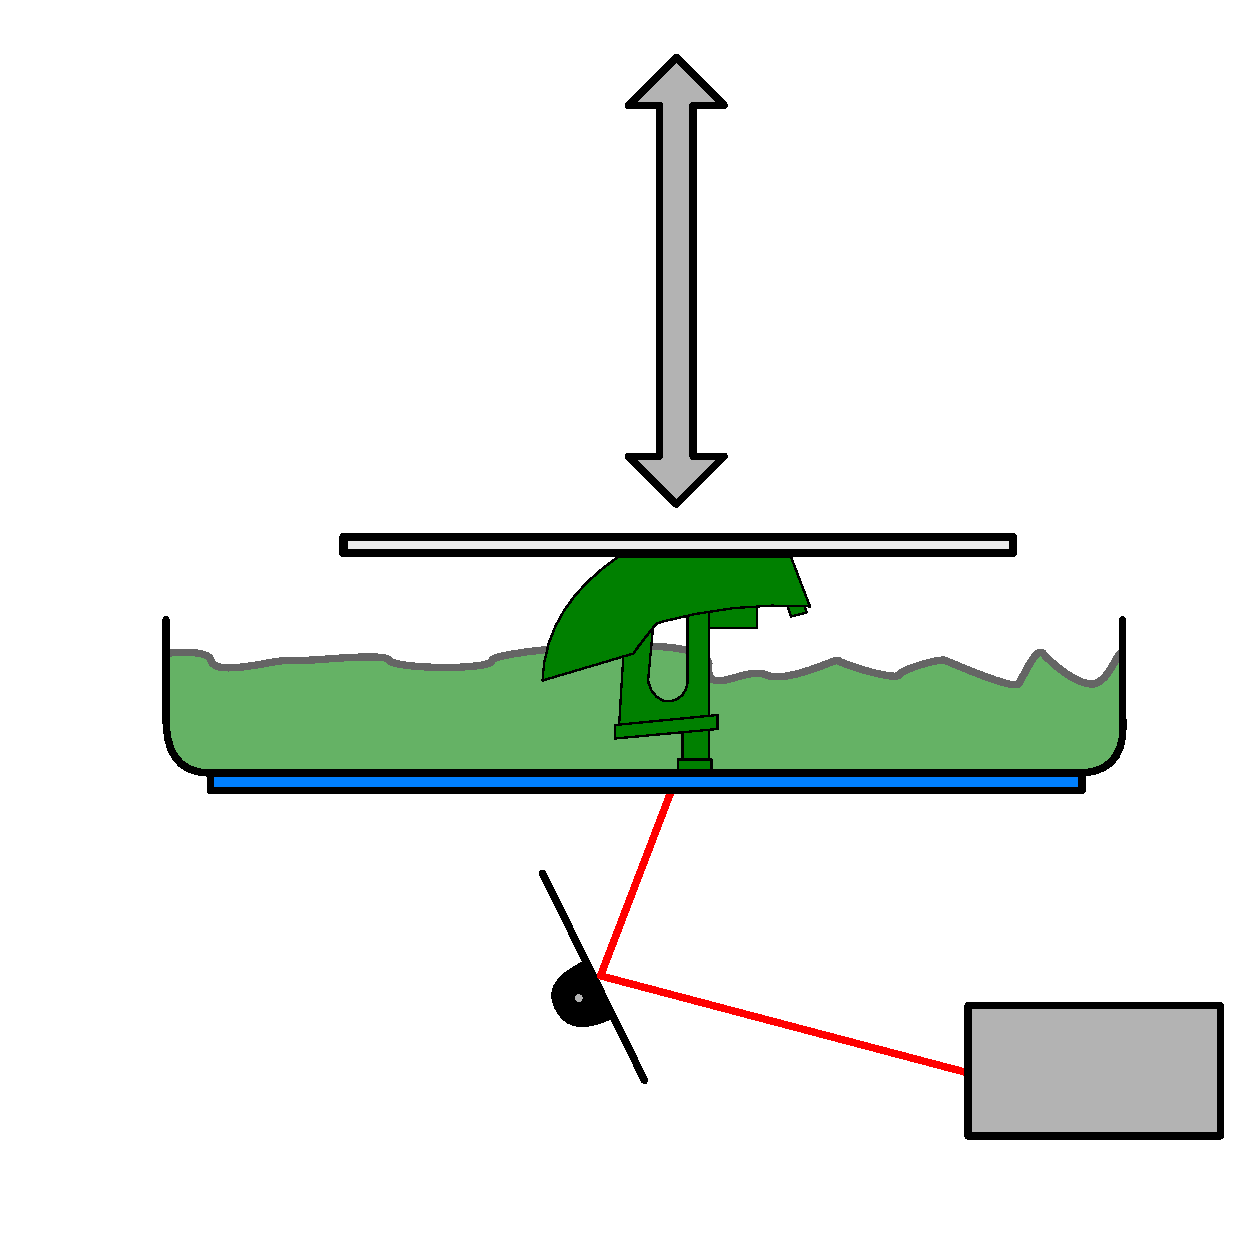
\includegraphics[width=0.6\textwidth, trim = 0px 45px 0px 10px, clip]{./bilder/SLA.pdf}
\end{center}

Verwenden Resin welches durch Licht ausgehärtet wird. \\
(Teuer. Kosten 80-100€ pro Liter.)


\newpage
\subsubsection{FDM (Fused Deposition Modeling) - Drucker}
\begin{center}
  \vspace{-1,7cm}
  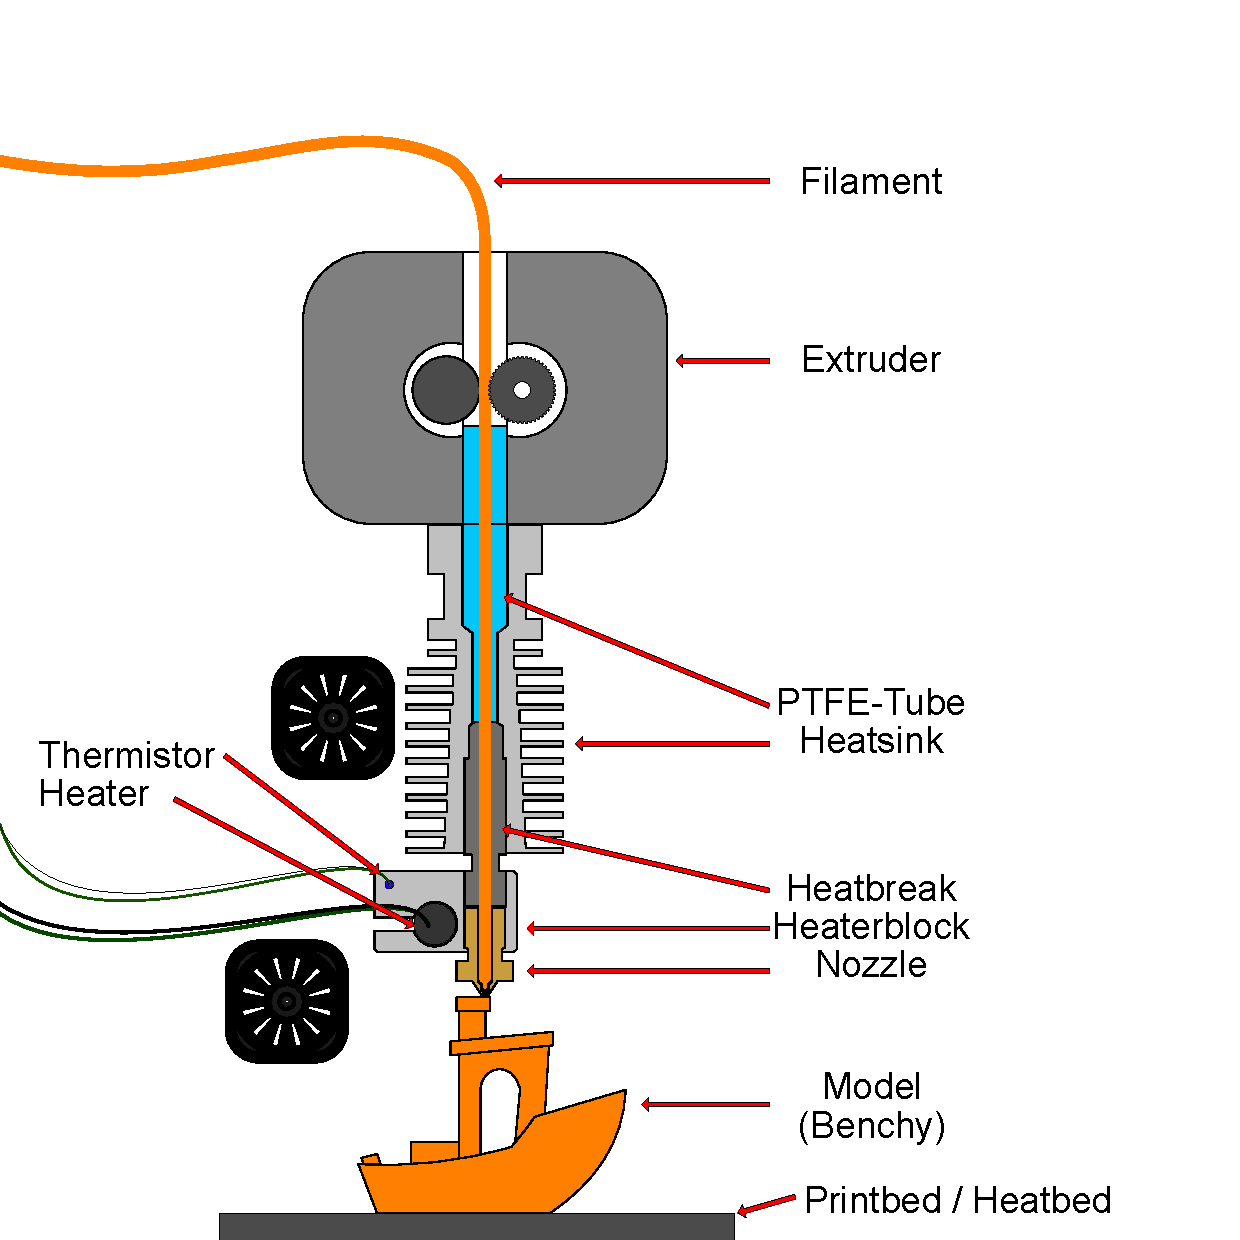
\includegraphics[width=0.6\textwidth]{./bilder/3dprinting.pdf}
\end{center}
Verwenden Filament auf Spulen.\\
(Kosten 13+ € pro Kilo / wobei gutes Filament bei 18€ anfängt)


\newpage % =
 % Geschichte und Arten
\subsection{Bauformen von FDM Druckern}
\begin{itemize}
  \item Karthesisch
  \item CoreXY
  \item Delta
  \item Polar
  \item Hangprinter
\end{itemize}


\newpage % ==================================================================

\begin{figure}[ht]
  \subsubsection{Karthesisch}
  % \section{Sensor - Varianten}
  % \subsection{Andere Ansätze fürs Bedleveling}


\adjustbox{valign=t}{\begin{minipage}[t]{0.45\textwidth}
\begin{framed}
  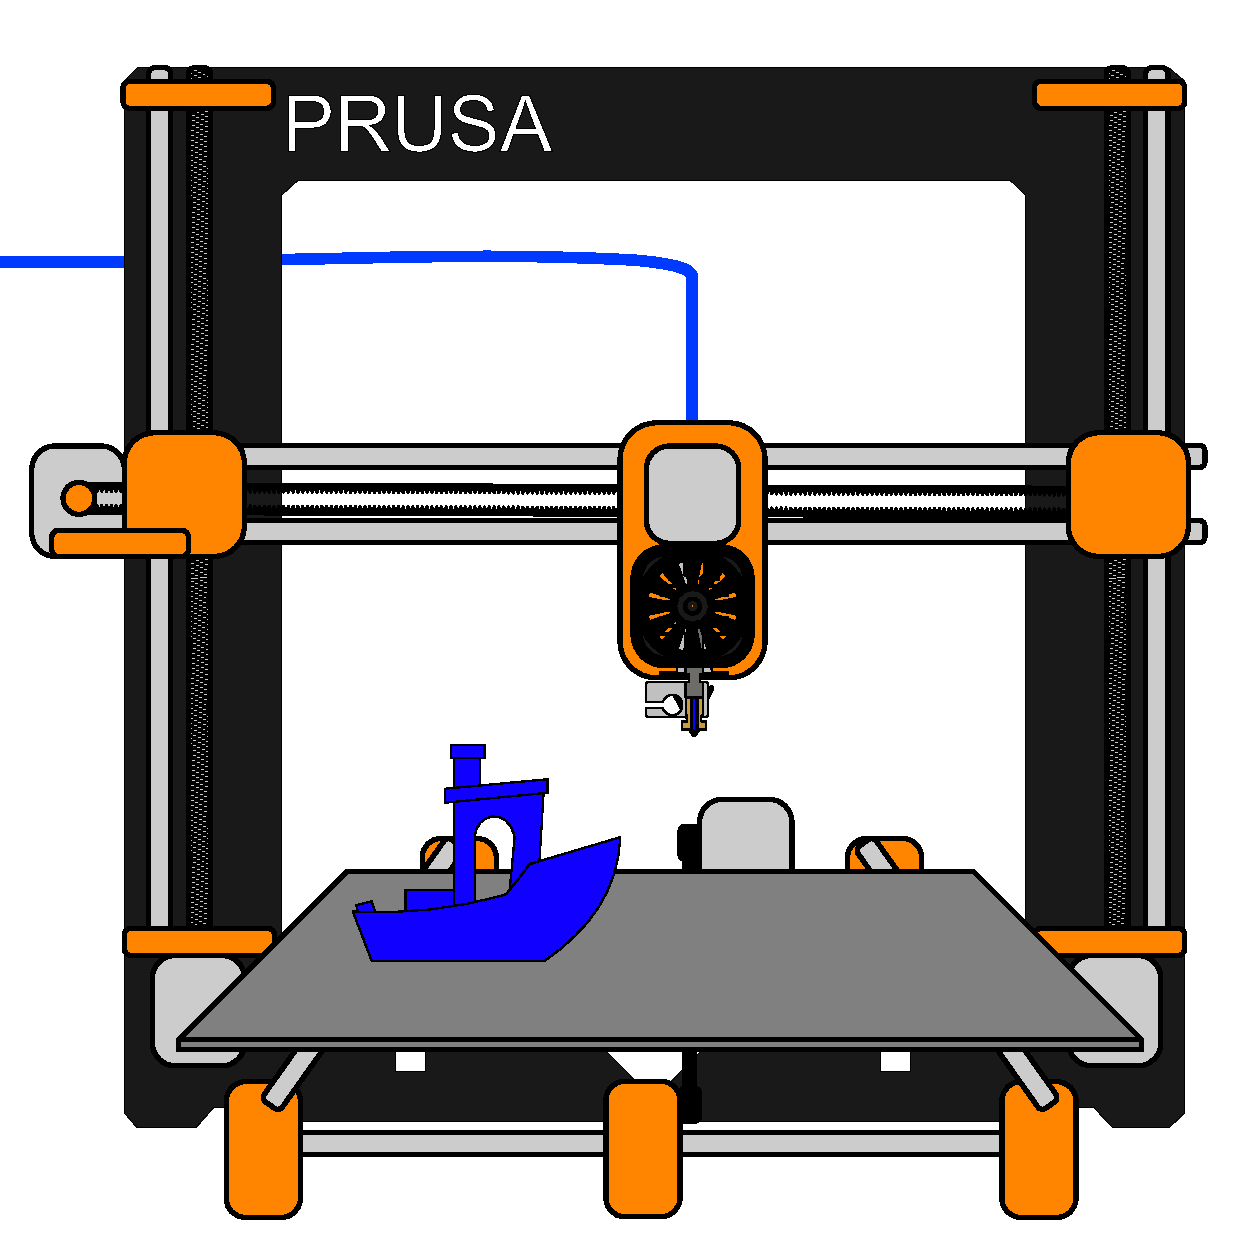
\includegraphics[width=1.0\textwidth, trim = 0px 0px 0px 0px, clip]{./bilder/karthesian.pdf}
\end{framed}

\end{minipage}}
% \hfill
\adjustbox{valign=t}{\begin{minipage}[t]{0.50\textwidth}
\vspace{0pt}
\huge
\hfill{}\textbf{karthesischer Drucker}\\

(Vom Prinzip her auch ein \\
karthesischer Drucker) \\

\vspace{0.2cm}

\textbf{Vorteile:}
\begin{itemize}
  \item Einfach zu bauen.
  \item Fehlerquellen relativ einfach zu finden.
\end{itemize}
\textbf{Nachteile:}
\begin{itemize}
  \item Layershifting
  \item Bei i3 Bauweise bewegendes Druckbed.
\end{itemize}
\end{minipage}}
\end{figure}
\clearpage % GleitObjekte anzeigen





% \subsubsection{Karthesisch}
% \begin{center}
%   \vspace{-2cm}
%   \hfill{}
%   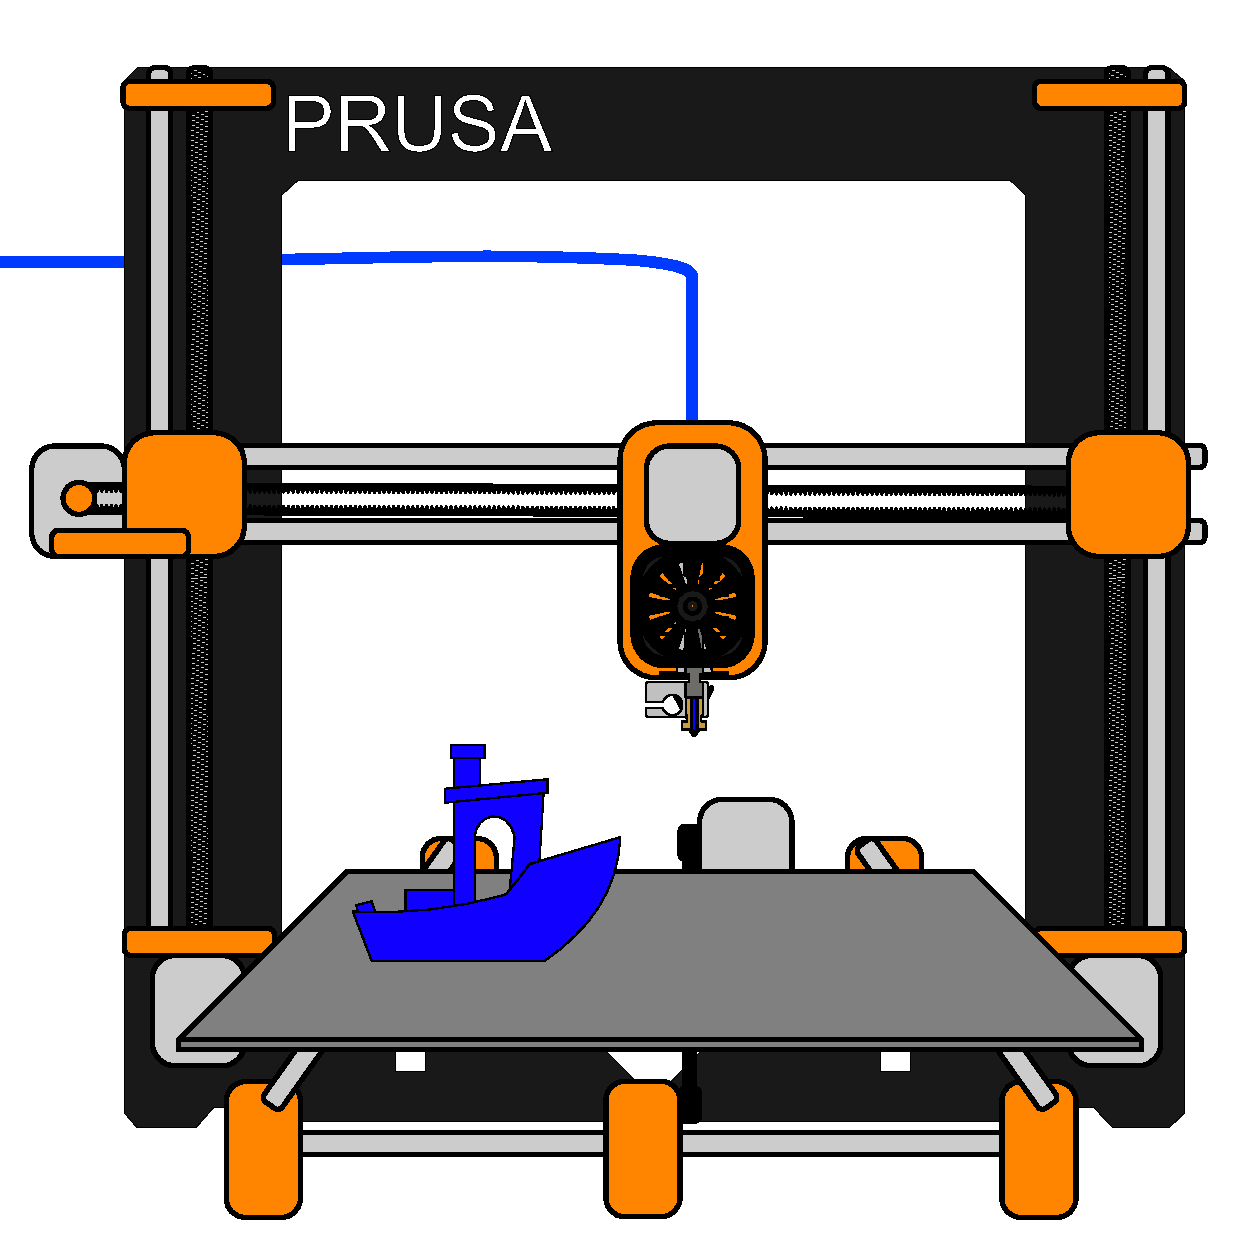
\includegraphics[width=0.4\textwidth]{./bilder/karthesian.pdf}
% \end{center}
% Vorteile:
% \begin{itemize}
%   \item Einfach zu bauen.
%   \item Fehlerquellen relativ einfach zu finden.
% \end{itemize}
% Nachteile:
% \begin{itemize}
%   \item Layershifting
%   \item Bei i3 Bauweise bewegendes Druckbed.
% \end{itemize}

\newpage % ==================================================================

\begin{figure}[ht]
  \subsubsection{CoreXY}
  % \section{Sensor - Varianten}
  % \subsection{Andere Ansätze fürs Bedleveling}


\adjustbox{valign=t}{\begin{minipage}[t]{0.45\textwidth}
\begin{framed}
  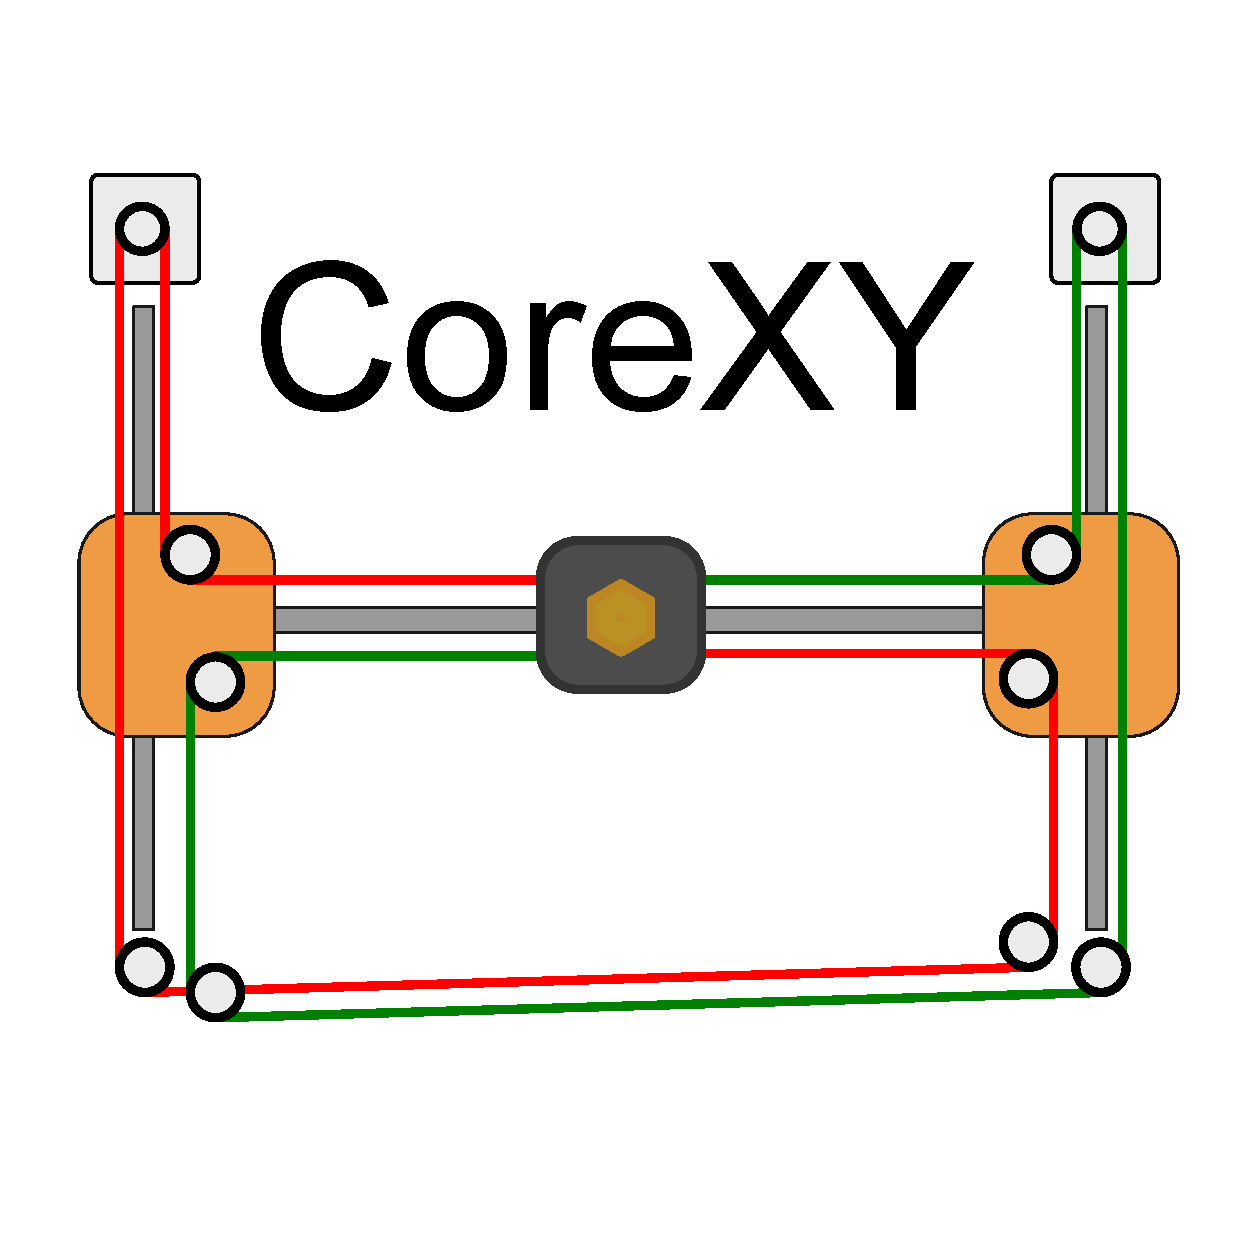
\includegraphics[width=1.0\textwidth, trim = 0px 0px 0px 0px, clip]{./bilder/CoreXY.pdf}
\end{framed}

\end{minipage}}
% \hfill
\adjustbox{valign=t}{\begin{minipage}[t]{0.50\textwidth}
\vspace{0pt}
\huge
\hfill{}\textbf{CoreXY - Drucker}\\

(Vom Prinzip her auch ein \\
karthesischer Drucker) \\

\vspace{0.2cm}

\textbf{Vorteile:}
\begin{itemize}
  \item Relativ einfach zu bauen.
  \item Fehlerquellen (relativ) einfach zu finden.
  \item Festes Druckbed \\$\Rightarrow$ bewegt sich nur in Z Achse.
\end{itemize}
\textbf{Nachteile:}
\begin{itemize}
  \item Layershifting
\end{itemize}
\end{minipage}}
\end{figure}
\clearpage % GleitObjekte anzeigen


% \subsubsection{CoreXY}
% \begin{center}
%   \vspace{-4cm}
%   \hfill{}
%   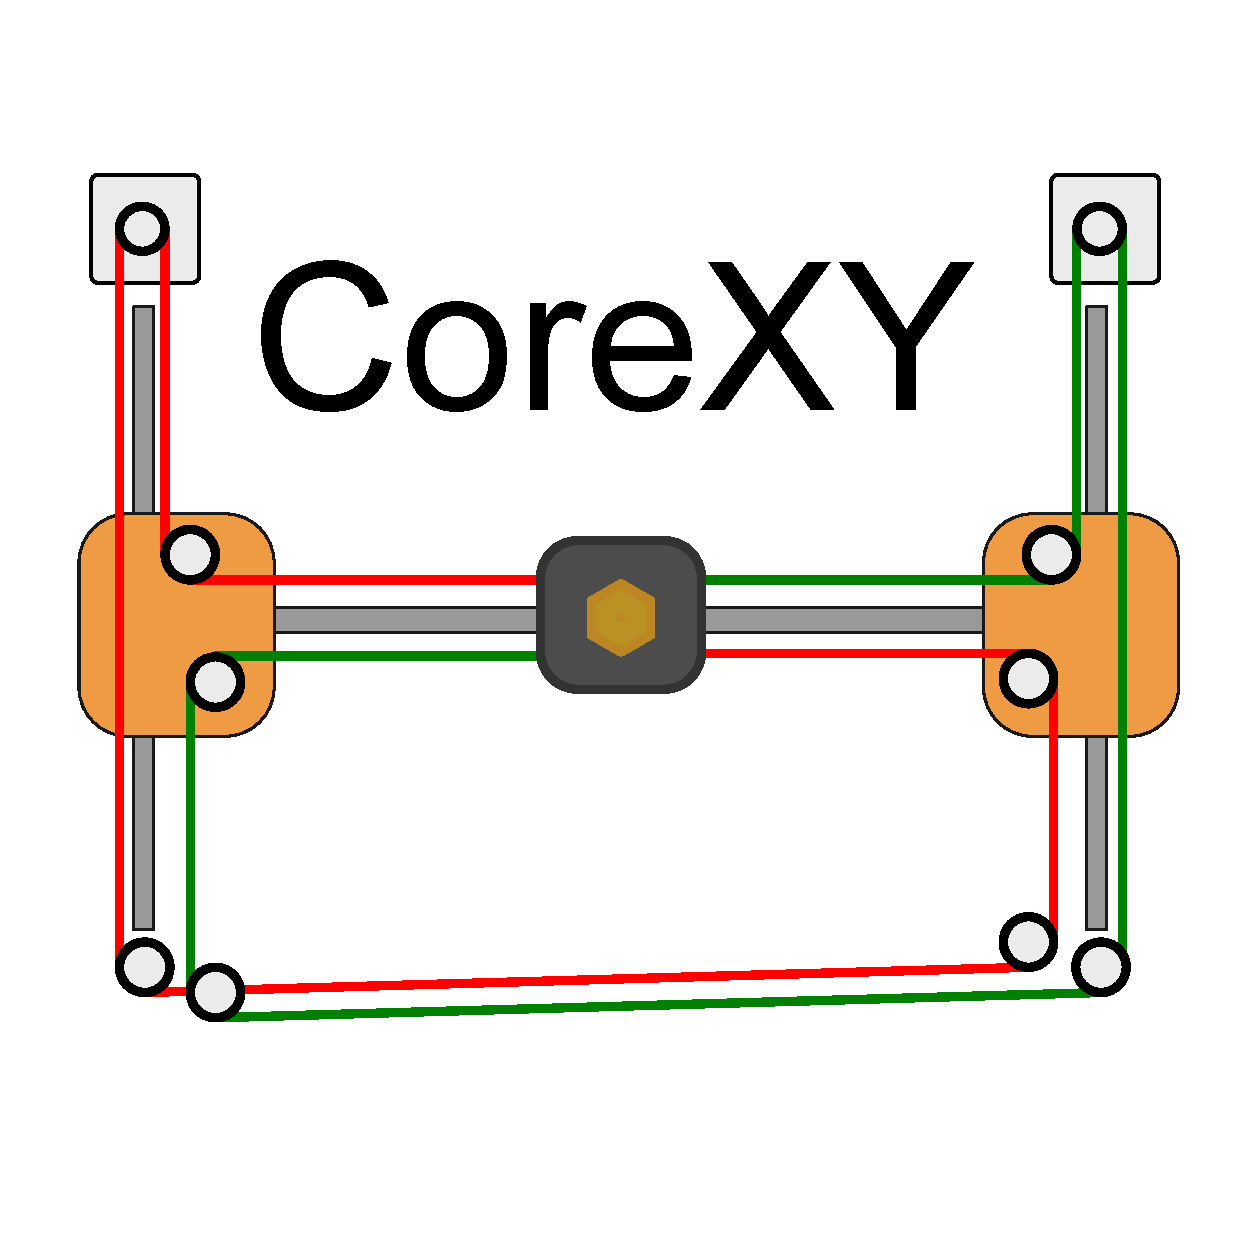
\includegraphics[width=0.5\textwidth]{./bilder/CoreXY.pdf}
% \end{center}
%
% (Vom Prinzip her auch ein karthesischer Drucker)
% Vorteile:
% \begin{itemize}
%   \item Relativ einfach zu bauen.
%   \item Fehlerquellen (relativ) einfach zu finden.
%   \item Festes Druckbed $\Rightarrow $bewegt sich nur in Z Achse.
% \end{itemize}
% Nachteile:
% \begin{itemize}
%   \item Layershifting
% \end{itemize}

\newpage % ==================================================================

% \subsubsection{Delta}
% \begin{center}
%   \vspace{-3cm}
%   \hfill{}
%   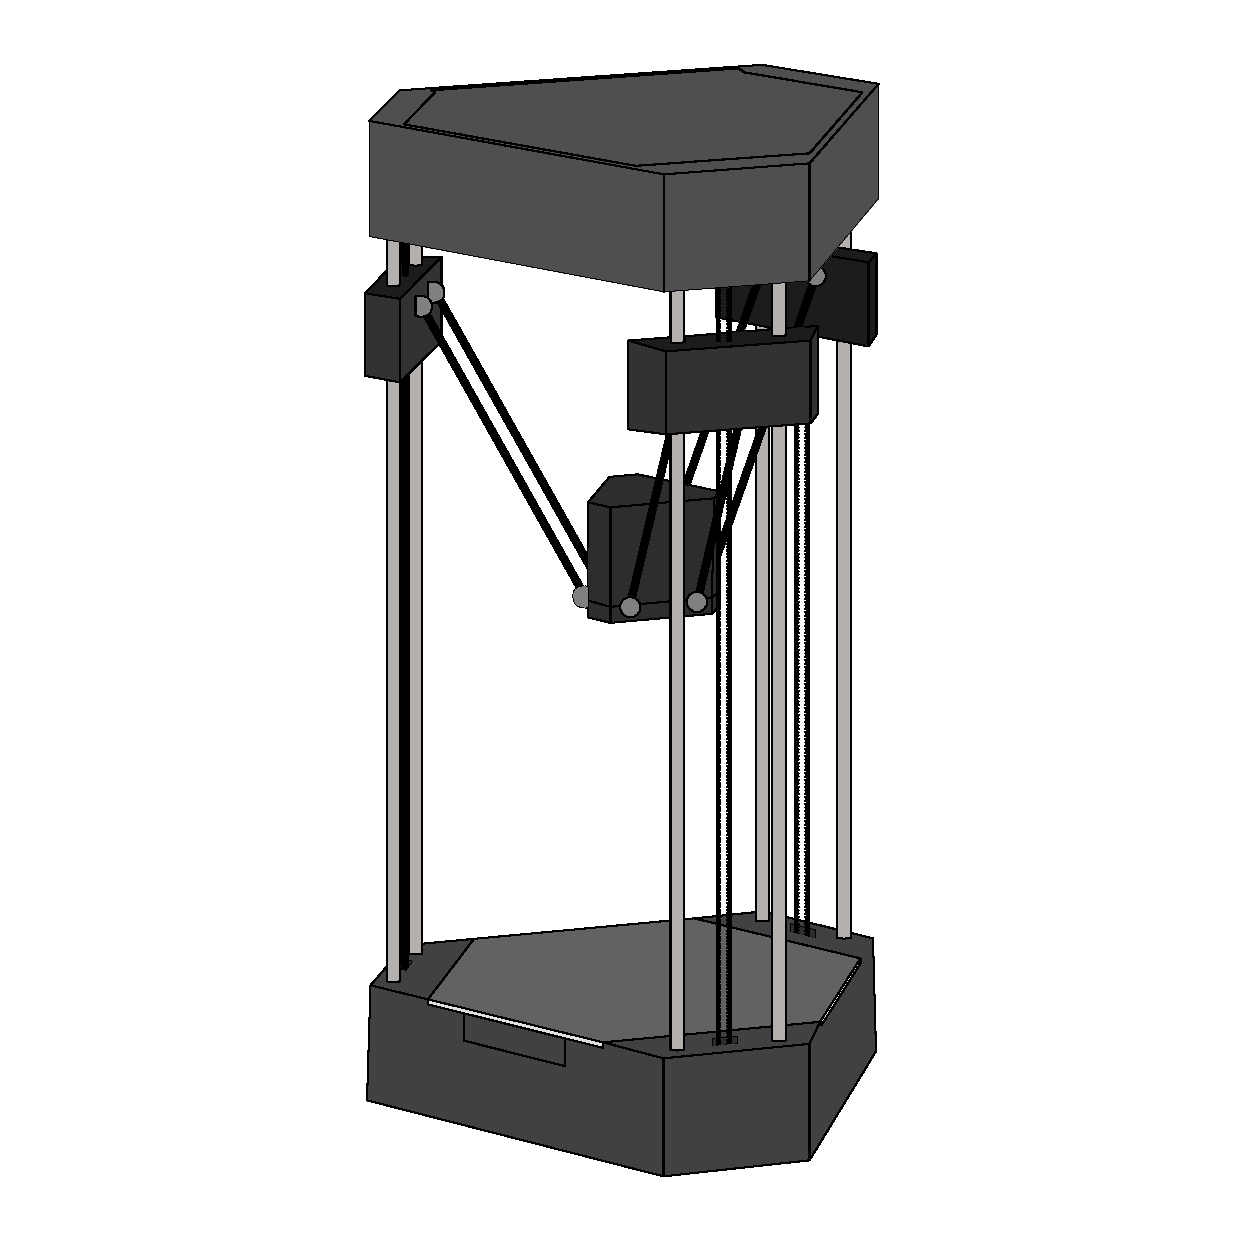
\includegraphics[width=0.5\textwidth]{./bilder/FLUXX.pdf}
% \end{center}

\begin{figure}[ht]
  \subsubsection{Delta}
  % \section{Sensor - Varianten}
  % \subsection{Andere Ansätze fürs Bedleveling}


\adjustbox{valign=t}{\begin{minipage}[t]{0.45\textwidth}
\begin{framed}
  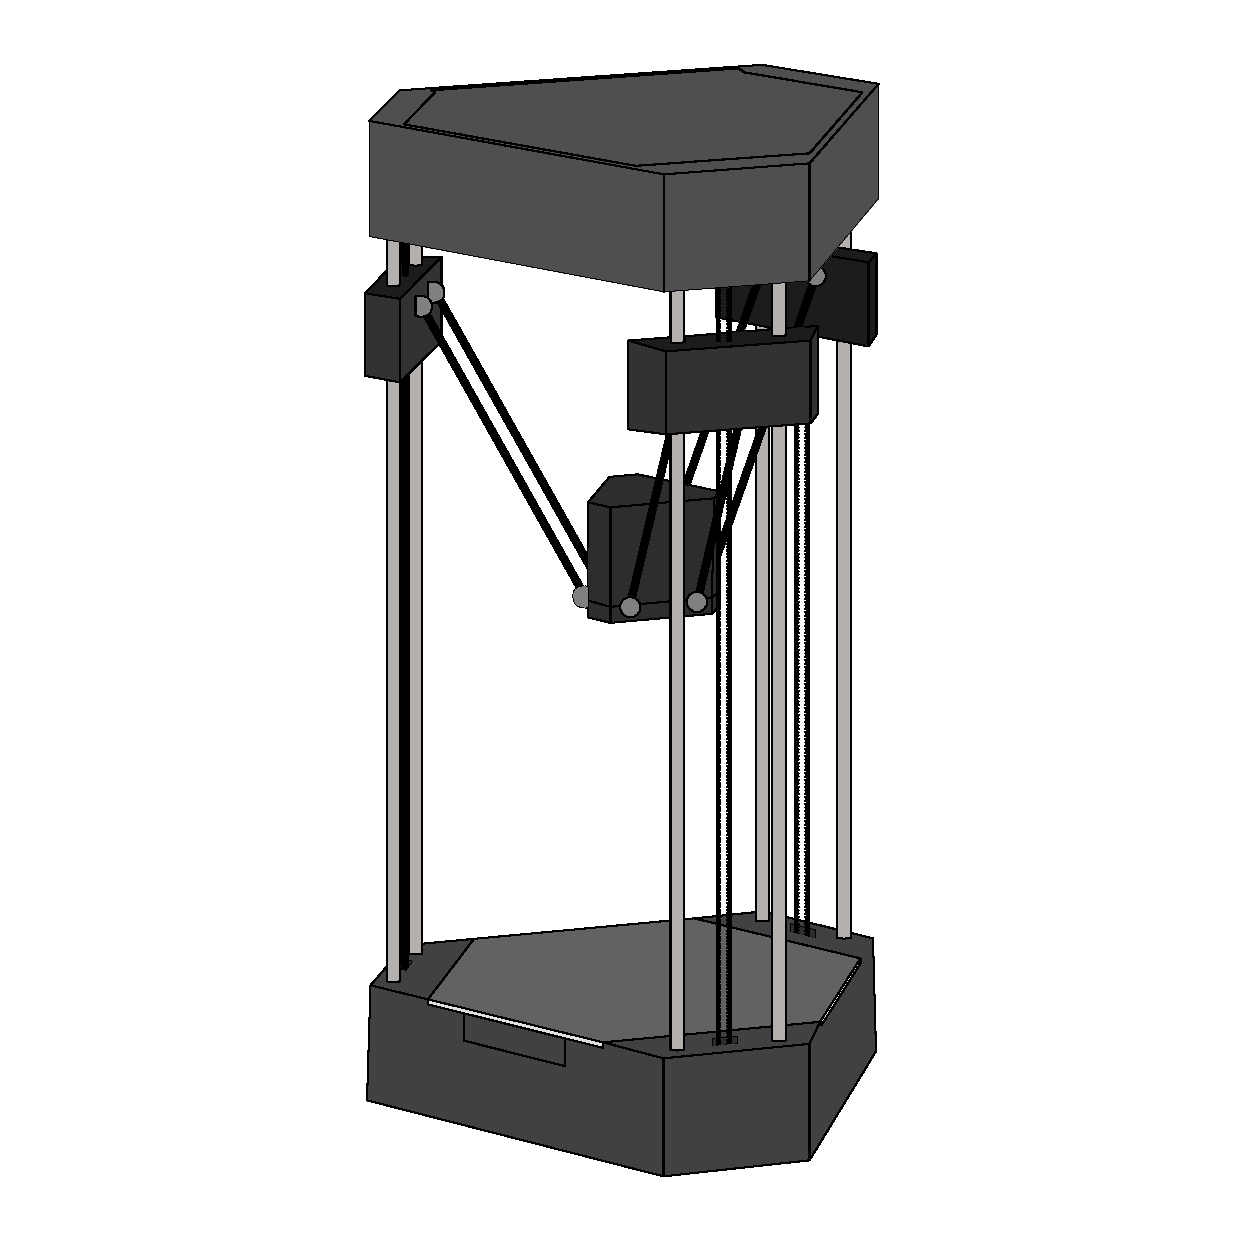
\includegraphics[width=1.0\textwidth, trim = 0px 0px 0px 0px, clip]{./bilder/FLUXX.pdf}
\end{framed}

\end{minipage}}
% \hfill
\adjustbox{valign=t}{\begin{minipage}[t]{0.50\textwidth}
\vspace{0pt}
\huge
\hfill{}\textbf{Flux Delta}
\begin{itemize}
  \item Leveling über Drucksensoren unterhalb des Printbed durch Berührung mit sauberer Düse. 
  \item Bei diesem Modell durch Closed Source Software kein Heatbed möglich.
  \item Delta haben in der Regel ein Bowden Setup
  \subitem Dadurch ist prinzipiell eine hohe Druckgeschwindigkeit möglich.
  \subitem \textbf{ABER}
  \subitem Delta Drucker haben meinstens keinen Partcooler \\ Dadurch sind wiederum nur langsame Geschwindigkeiten Sinnvoll.
\end{itemize}
\end{minipage}}
\end{figure}
\clearpage % GleitObjekte anzeigen

\newpage % ==================================================================


% \subsubsection{Polar}
\begin{figure}[ht]
  \subsubsection{Polar}
  % \section{Sensor - Varianten}
  % \subsection{Andere Ansätze fürs Bedleveling}


\adjustbox{valign=t}{\begin{minipage}[t]{0.45\textwidth}
\begin{framed}
  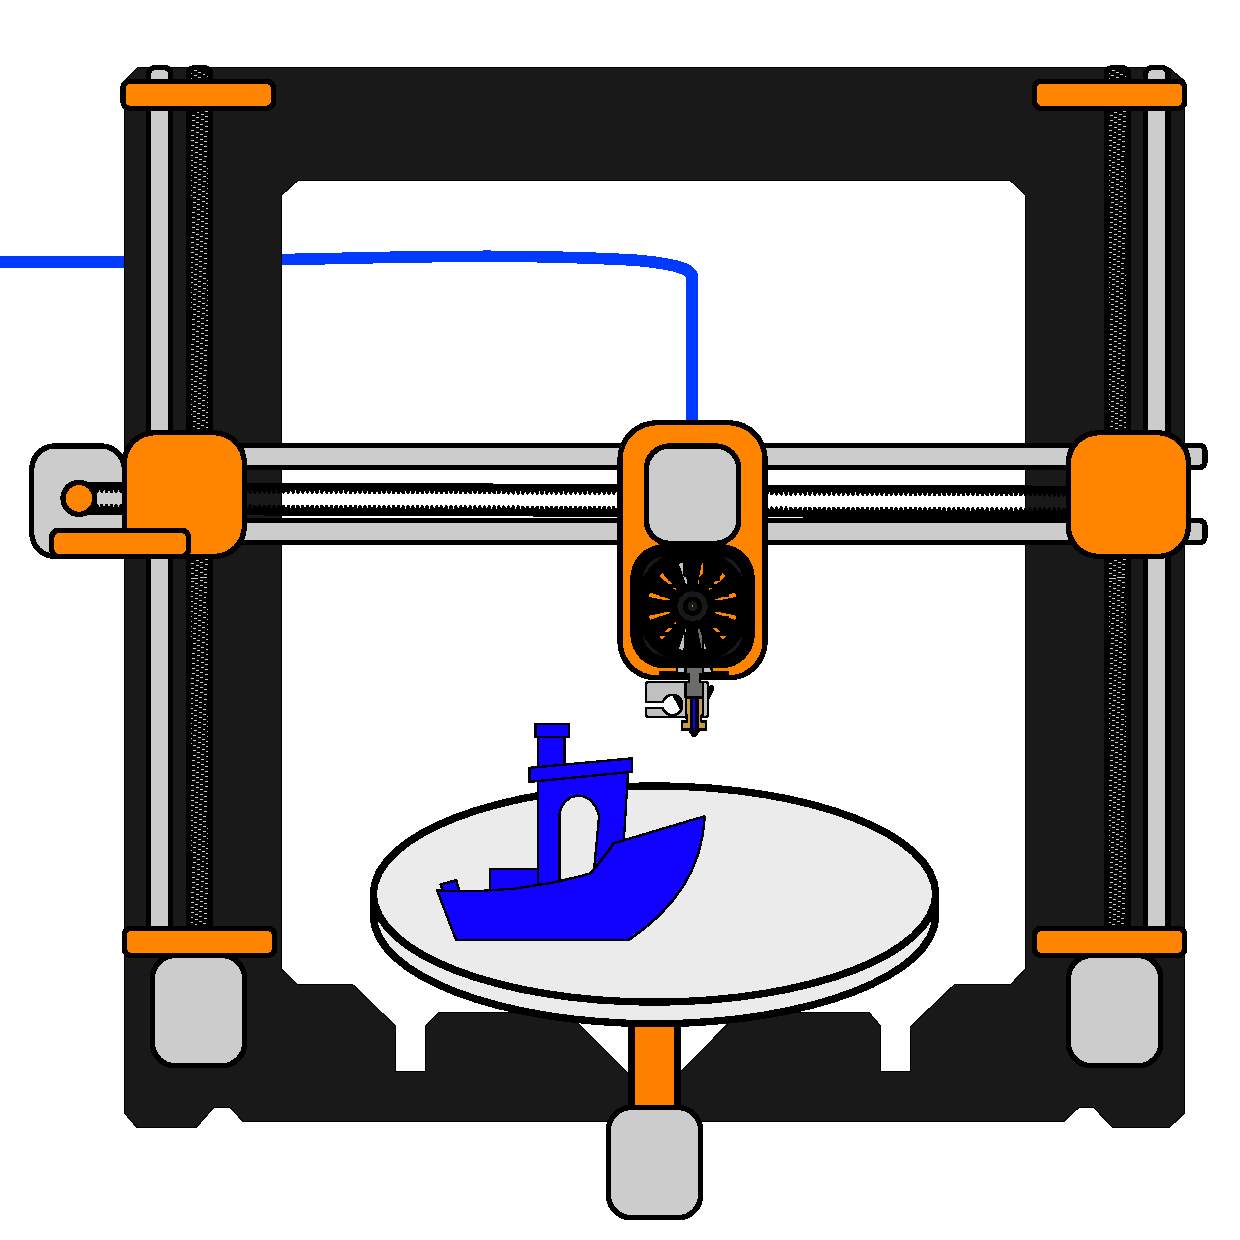
\includegraphics[width=1.0\textwidth, trim = 0px 0px 0px 0px, clip]{./bilder/Polar.pdf}
\end{framed}

\end{minipage}}
% \hfill
\adjustbox{valign=t}{\begin{minipage}[t]{0.50\textwidth}
\vspace{0pt}
\huge
\hfill{}\textbf{Polarer Drucker}\\
\vspace{-0.5cm}
\begin{center}
  \Huge{\textbf{Achtung ab hier nur noch Sarkasmus !!!}}
\end{center}
\textbf{Vorteile:}
\begin{itemize}
  \item Joah !!! \\ Eigentlich nur gut für Vasen.
  \item Man kann 4 Kästen Bier während der Fehlersuche trinken.
  \item Druckbed ist super stabil.
\end{itemize}
\begin{center}
  \Huge{\textbf{Nein, im Ernst einen solchen Drucker sollte man nur bauen wenn man zu viel Zeit hat.}}
\end{center}
% \textbf{Nachteile:}
\end{minipage}}
\end{figure}
\clearpage % GleitObjekte anzeigen

\newpage % ==================================================================

\begin{figure}[ht]
  \subsubsection{HangPrinter}
  % \section{Sensor - Varianten}
  % \subsection{Andere Ansätze fürs Bedleveling}


\adjustbox{valign=t}{\begin{minipage}[t]{0.5\textwidth}
\begin{framed}
  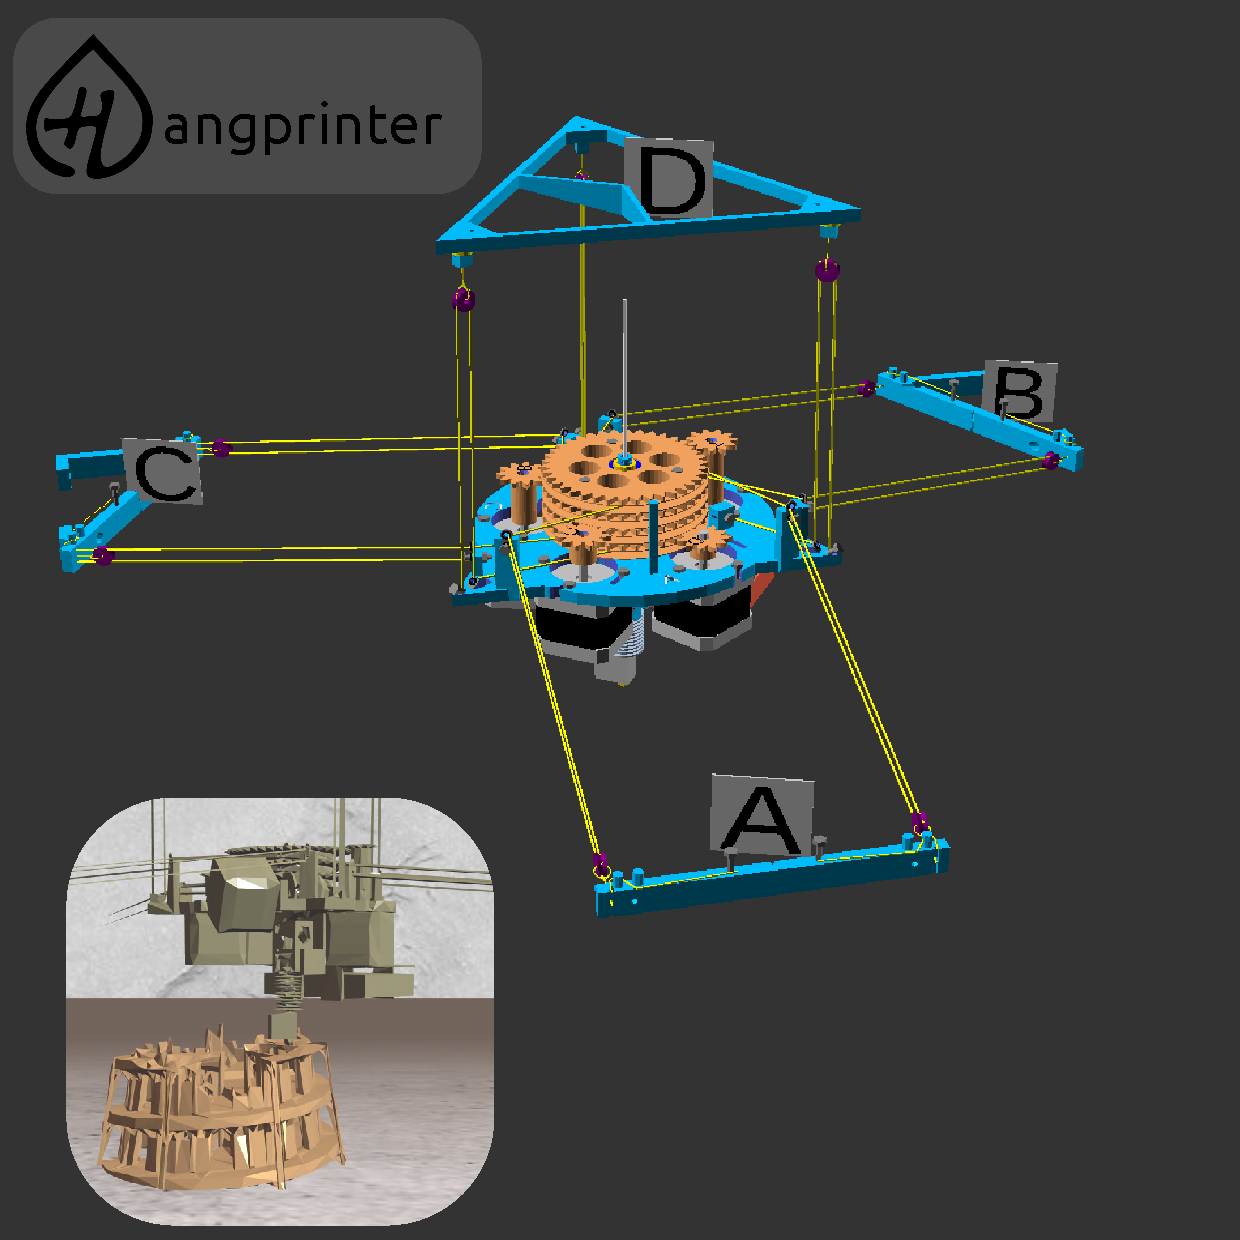
\includegraphics[width=1.0\textwidth, trim = 0px 0px 0px 0px, clip]{./bilder/Hangprinter.pdf}
\end{framed}

\end{minipage}}
% \hfill
\adjustbox{valign=t}{\begin{minipage}[t]{0.45\textwidth}
\vspace{0pt}
\huge
\hfill{}\textbf{HangPrinter}\\
\vspace{-0.5cm}
\begin{center}
  (Spiderman, Spiderman ...)
\end{center}
\vspace{0.2cm}

\textbf{Vorteile:}
\begin{itemize}
  \item Bauraum bis einen die \\ Erdkrümmung kickt.
  \item Keine blöden Bauteile \\ (Wie Gewindestangen, \\Gurte, ...)
\end{itemize}
\textbf{Nachteile:}
\begin{itemize}
  \item Es gibt bisher nur einen.
  \item Relativ wenig doku.
  \item Höchst experimentell.
  \item Nach ca. 1 Meter muss man den Druck pausieren und neu kalibrieren.
\end{itemize}
\end{minipage}}
\end{figure}
\clearpage % GleitObjekte anzeigen

\newpage % ==================================================================





% \vspace{0.5cm}
%
% \begin{center}
%   \includegraphics[width=1.0\textwidth]{./bilder/plainRepo.png}
% \end{center}

%
%
% \begin{figure}[]
%   \subsubsection{Github Repo mit Travis CI verbinden}
% \adjustbox{valign=t}{\begin{minipage}[t]{0.50\textwidth}
% \begin{framed}
%   \includegraphics[width=1.0\textwidth]{./bilder/1gitRepoSettings.png}
% \end{framed}
%
% \end{minipage}}
% % \hfill
% \adjustbox{valign=t}{\begin{minipage}[t]{0.5\textwidth}
% \vspace{0pt}
% \huge
% Im Repo klickt man auf Settings
% % \caption{Kapazität}
% \end{minipage}}
% % \end{figure}
% % \vspace{0.5cm} % ----------------------------------- vspace
% % \begin{figure}[ht]
% \adjustbox{valign=t}{\begin{minipage}[t]{0.40\textwidth}
% % \vspace{0.5cm}
% \begin{framed}
%   \includegraphics[width=1.0\textwidth]{./bilder/2integrationServices.png}
% \end{framed}
%
% \end{minipage}}
% \hfill
% \adjustbox{valign=t}{\begin{minipage}[t]{0.43\textwidth}
% \vspace{0pt}
% \huge
% Danach
% % \caption{Kapazität}
% \end{minipage}}
% \end{figure}
%
% \clearpage % GleitObjekte anzeigen
% \newpage
% \begin{table}
%   \caption{title}
% \end{table}
% Test


% \begin{center}
%  % \includegraphics[scale=0.5]{./pictures/wohnzimmer.png}
% \end{center}
% \begin{figure}
%     \subfigure[Bezeichnung der linken Grafik]{\includegraphics[width=0.49\textwidth]{./bilder/1gitRepoSettings.png}}
%     \subfigure[Bezeichnung der rechten Grafik]{\includegraphics[width=0.49\textwidth]{./bilder/2integrationServices.png}}
% \caption{Titel unterm gesamten Bild}
% \end{figure}


% \begin{figure}
%     \subfigure[Bezeichnung der linken Grafik]{\includegraphics[width=0.49\textwidth]{./bilder/1gitRepoSettings.png}}
%     \subfigure[Bezeichnung der rechten Grafik]{Test tesxt}
% \caption{Titel unterm gesamten Bild}
% \end{figure}


%
% \section{Bauformen von 3D Druckern}
% as
% \subsection{Drucker nach Materialart}
% as
% \subsubsection{SLA}
% asas
% \subsubsection{FDM}
% asasas
% \subsection{Bauformen von FDM Druckern}
% \subsubsection{Karthesisch}
% \subsubsection{CoreXYZ}
% \subsubsection{Delta}
% \subsubsection{Hangprinter}
% \subsubsection{rotierend}
 %  Bauformen
\newpage % ============================================= Newpage ===================

\begin{figure}[ht]
  \section{Möglichkeiten der Ansteuerung des Druckers}

\adjustbox{valign=t}{\begin{minipage}[t]{0.45\textwidth}
\subsection{RAMPS 1.4}
\begin{framed}
  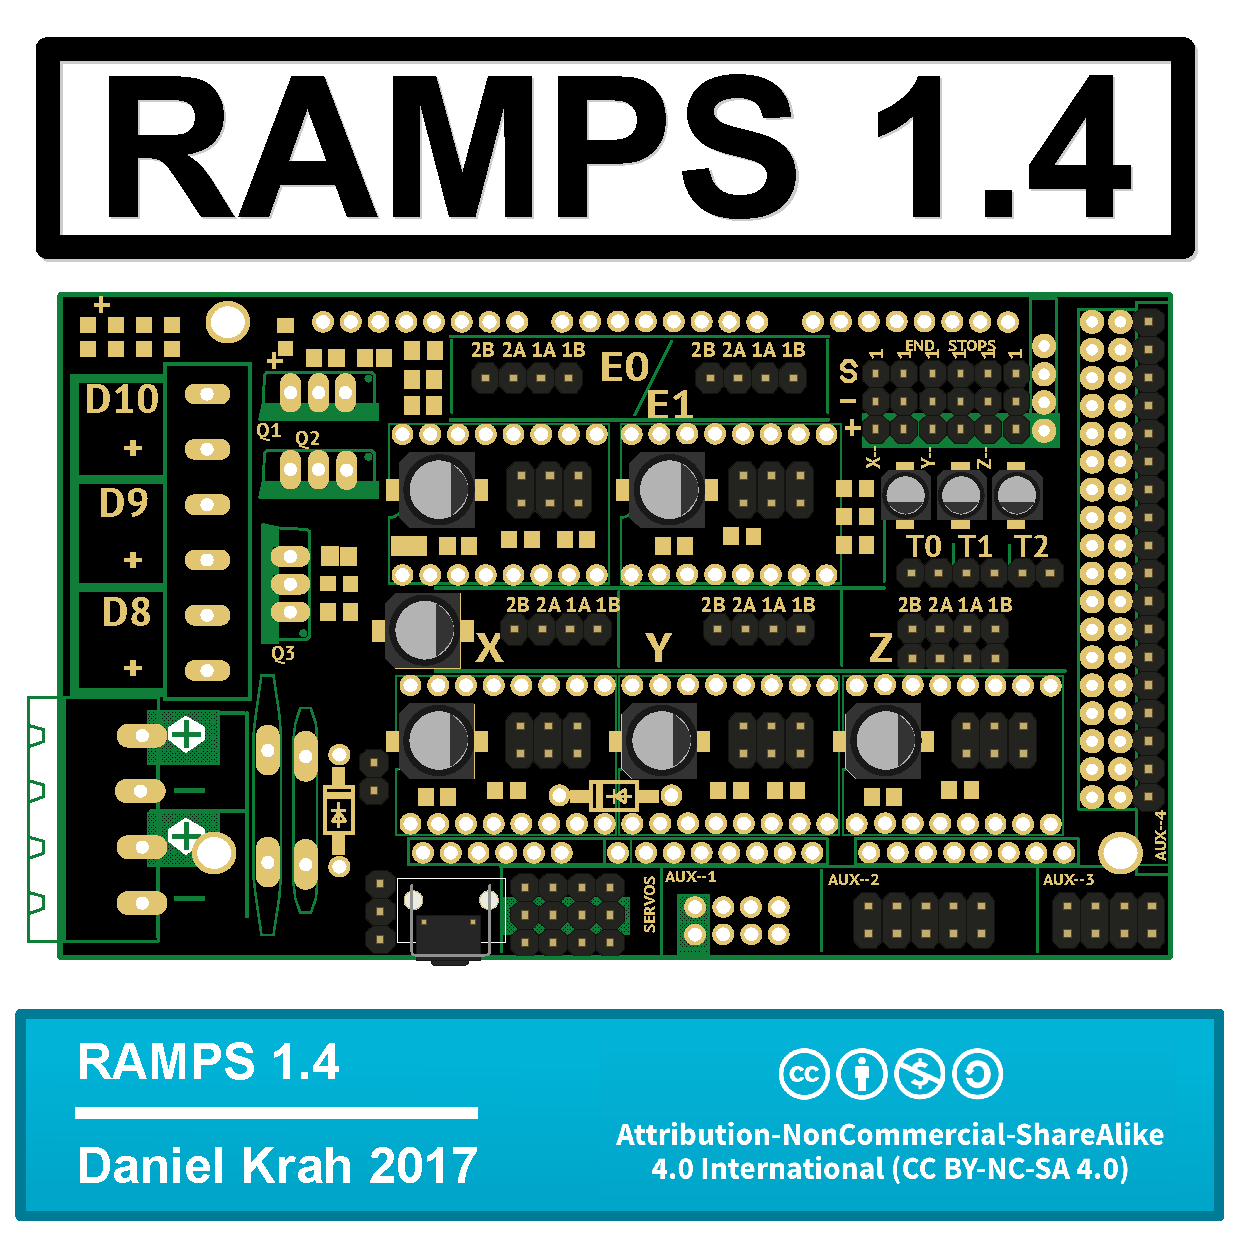
\includegraphics[width=1.0\textwidth, trim = 0px 0px 0px 0px, clip]{./bilder/RAMPS14.pdf}
\end{framed}
\end{minipage}}
% \hfill
\adjustbox{valign=t}{\begin{minipage}[t]{0.45\textwidth}
\subsection{SmoothieBoard}
\vspace{-0.34cm}
\begin{framed}
  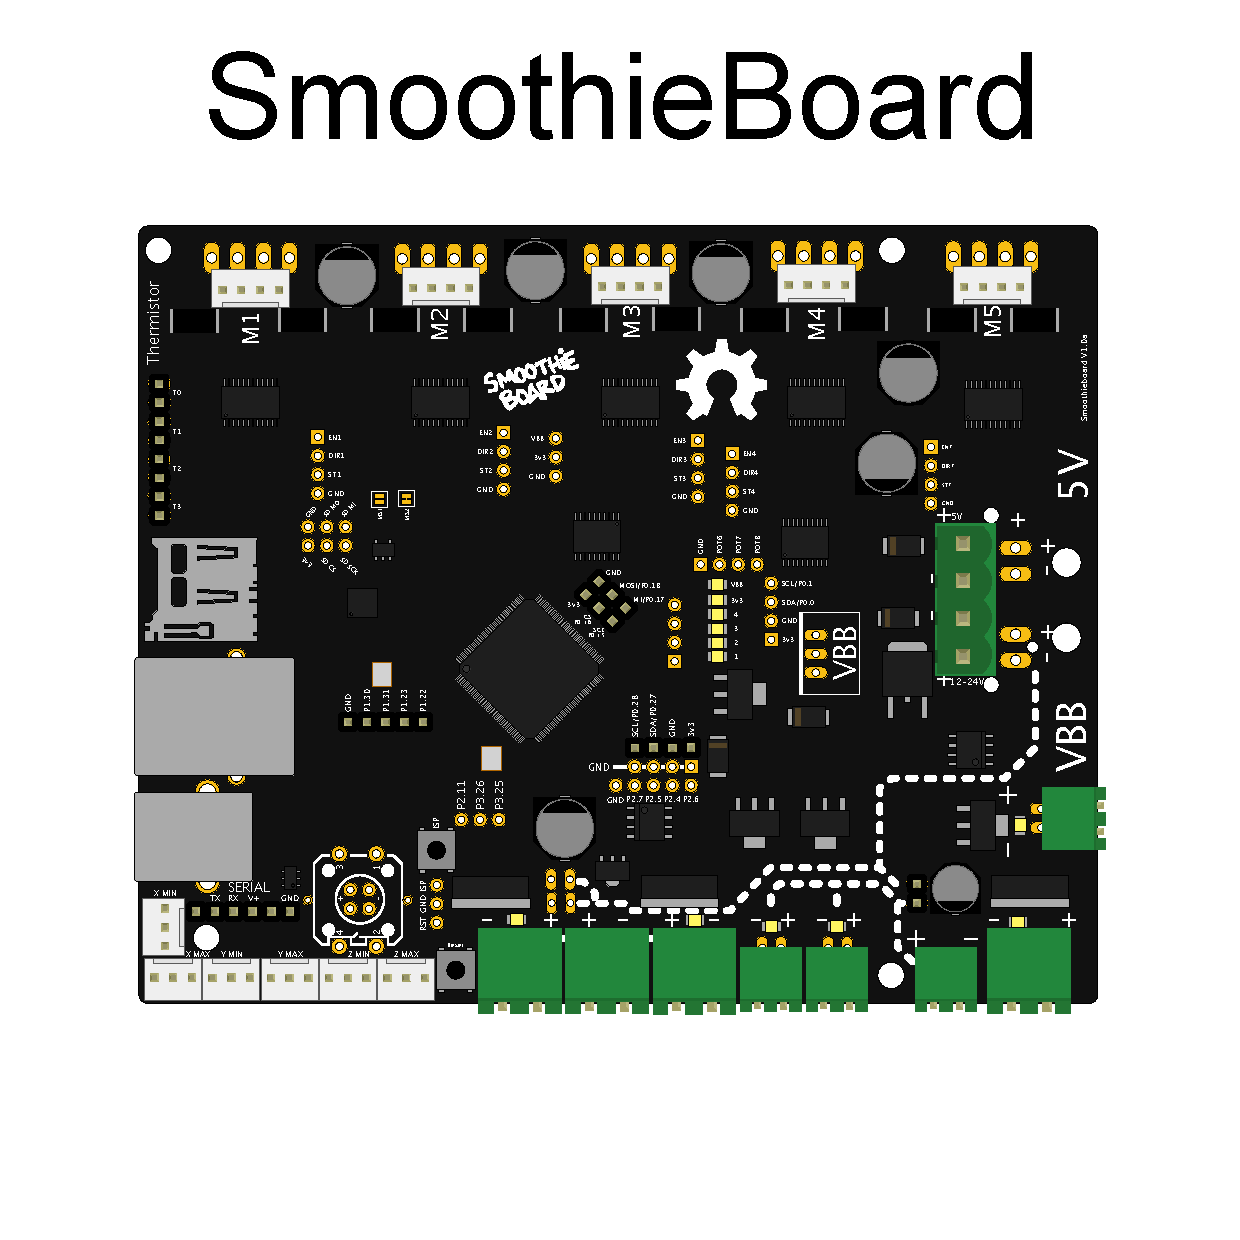
\includegraphics[width=1.0\textwidth, trim = 0px 0px 0px 0px, clip]{./bilder/SmoothieBoard.pdf}
\end{framed}
\end{minipage}}

% \hfill

\adjustbox{valign=t}{\begin{minipage}[t]{0.45\textwidth}
\vspace{0,3cm}
\huge
\textbf{Vorteile}
\begin{itemize}
  \item Extrem Billig \\(inkl. Arduino ca 12€)
  \item Große community
\end{itemize}
% \caption{Kapazität}
\end{minipage}}
% \end{figure}
% \vspace{0.5cm} % ----------------------------------- vspace
% \begin{figure}[ht]
% \hfill
\adjustbox{valign=t}{\begin{minipage}[t]{0.45\textwidth}
\vspace{0,3cm}
\huge
\textbf{Vorteile}
\begin{itemize}
  \item 32 Bit @ 120 MHz, \\ viel Flash und Ram
  \item Ethernet, 4 Temp.-Sensoren
  \item Mit Stepper-Driver bestückt
\end{itemize}

% \caption{Kapazität}
\end{minipage}}
\end{figure}

\clearpage % GleitObjekte anzeigen





\newpage % ============================================= Newpage ===================
% \vspace{-3cm}
\begin{figure}[ht]
  % \section{Möglichkeiten der Ansteuerung des Druckers}

\adjustbox{valign=t}{\begin{minipage}[t]{0.40\textwidth}
% \section{RAMPS 1.4}
\begin{framed}
  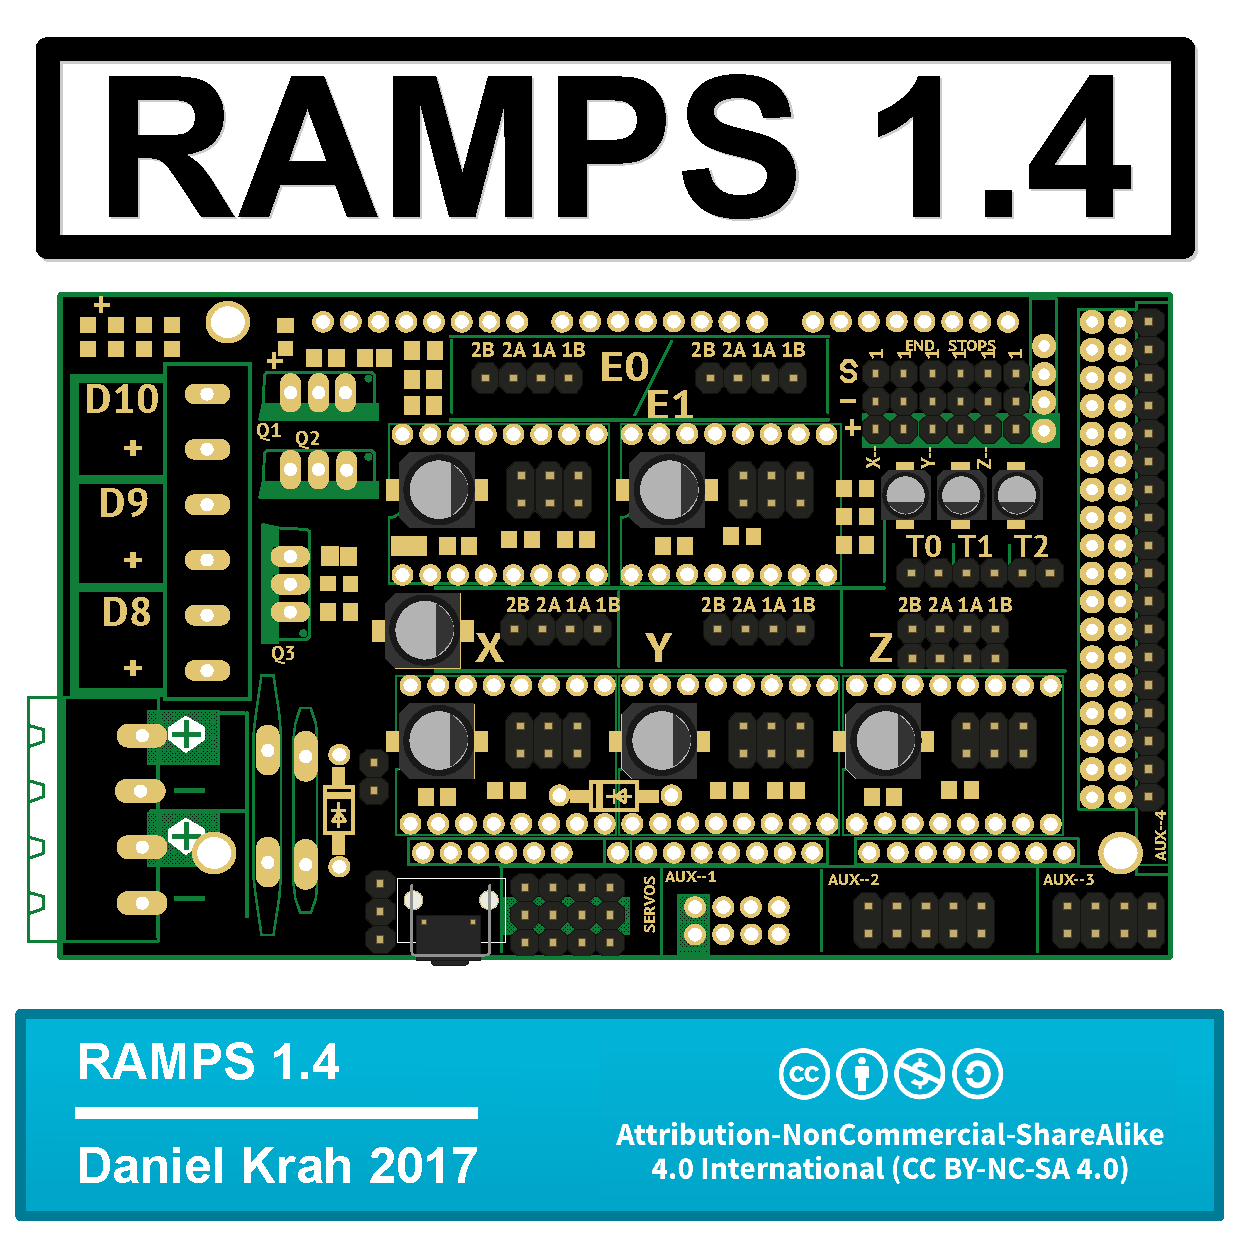
\includegraphics[width=1.0\textwidth, trim = 0px 0px 0px 0px, clip]{./bilder/RAMPS14.pdf}
\end{framed}
\end{minipage}}
% \hfill
\adjustbox{valign=t}{\begin{minipage}[t]{0.40\textwidth}
% \section{SmoothieBoard}
% \vspace{-0.34cm}
\begin{framed}
  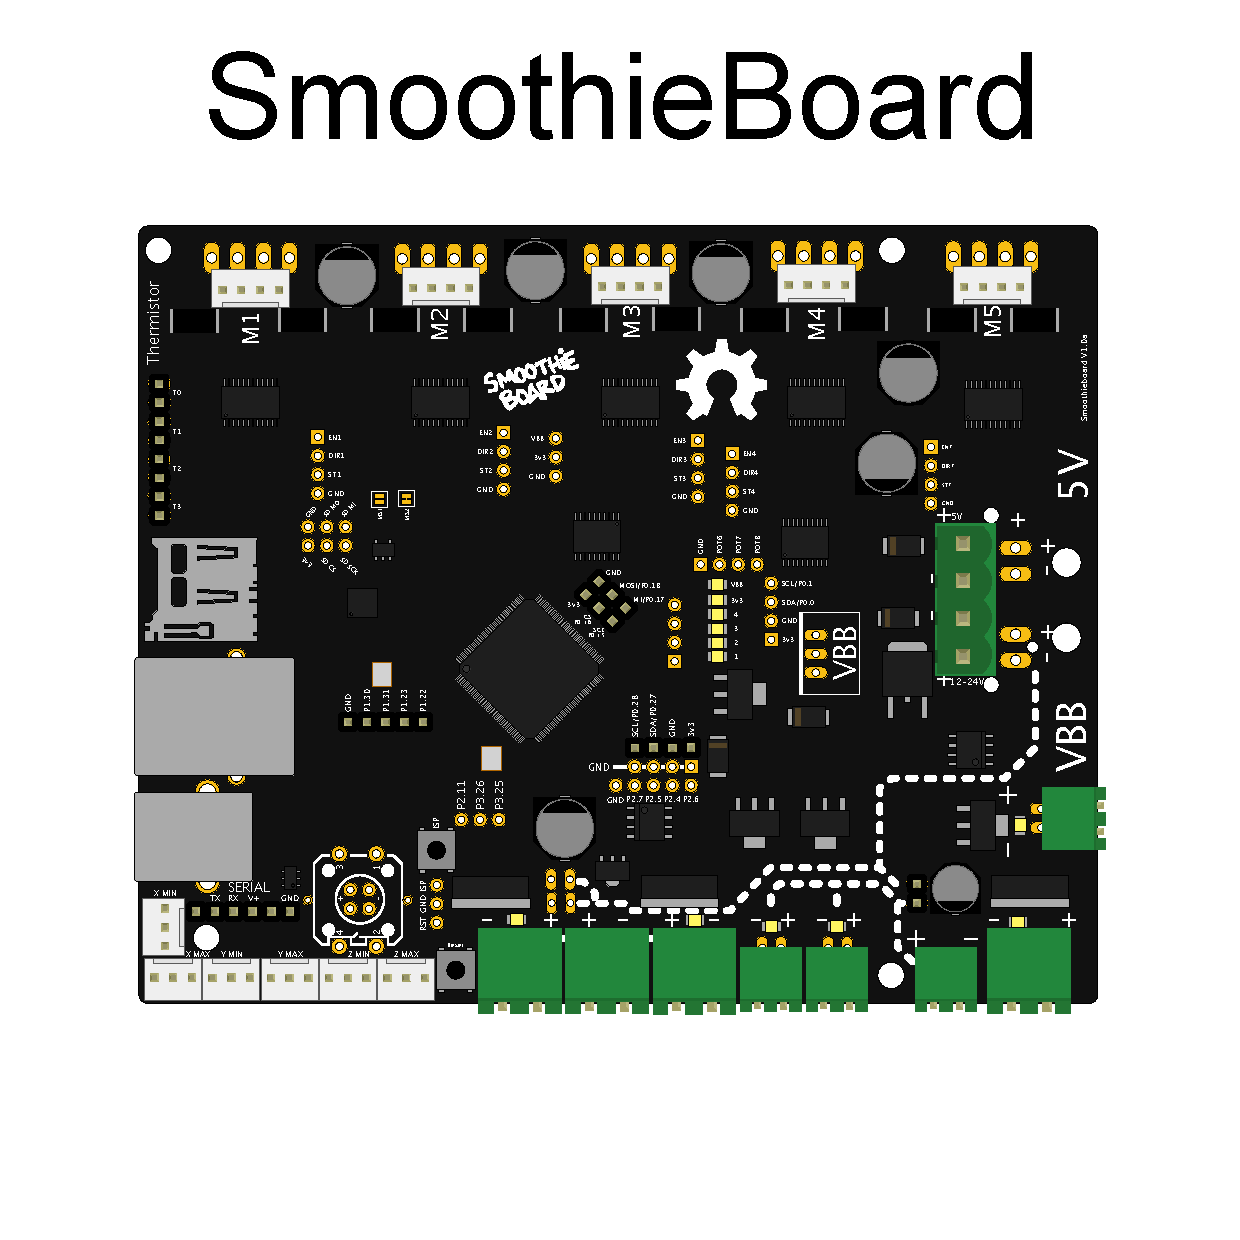
\includegraphics[width=1.0\textwidth, trim = 0px 0px 0px 0px, clip]{./bilder/SmoothieBoard.pdf}
\end{framed}
\end{minipage}}

% \hfill

\adjustbox{valign=t}{\begin{minipage}[t]{0.40\textwidth}
\vspace{0,3cm}
\huge
\textbf{Nachteile}
\begin{itemize}
  \item 8 Bit @ 12 MHZ
  \item Nur EEprom
  \item Wenig Ampere für \\ das Heatbed
  \item Brandgefahr !!! Die \\Stecker sind Schrott.
\end{itemize}
% \caption{Kapazität}
\end{minipage}}
% \end{figure}
% \vspace{0.5cm} % ----------------------------------- vspace
% \begin{figure}[ht]
% \hfill
\adjustbox{valign=t}{\begin{minipage}[t]{0.40\textwidth}
\vspace{0,3cm}
\huge
\textbf{Nachteile}
\begin{itemize}
  \item 32 Bit 120 MHz, \\viel Flash/Ram,
  \item Lan-Anschluss, \\4 Thermal-Sensoren
  \item Mit Stepper-Driver \\bestückt
\end{itemize}

% \caption{Kapazität}
\end{minipage}}
\end{figure}

\clearpage % GleitObjekte anzeigen

% Rampswire14


\newpage % ============================================= Newpage ===================

\begin{figure}[ht]
  % \section{Möglichkeiten der Ansteuerung des Druckers}

  \adjustbox{valign=t}{\begin{minipage}[t]{0.45\textwidth}
  \vspace{0,3cm}
  \huge
  \textbf{Open Hardware}\\
  Beide Boards sind Open Source.\\
  (Alle Abbildung RAMPS)
  % \caption{Kapazität}
  \end{minipage}}
  \hspace{-7cm}
  \adjustbox{valign=t}{\begin{minipage}[t]{0.45\textwidth}
  % \section{SmoothieBoard}
  % \vspace{-0.34cm}
  % \begin{framed}
    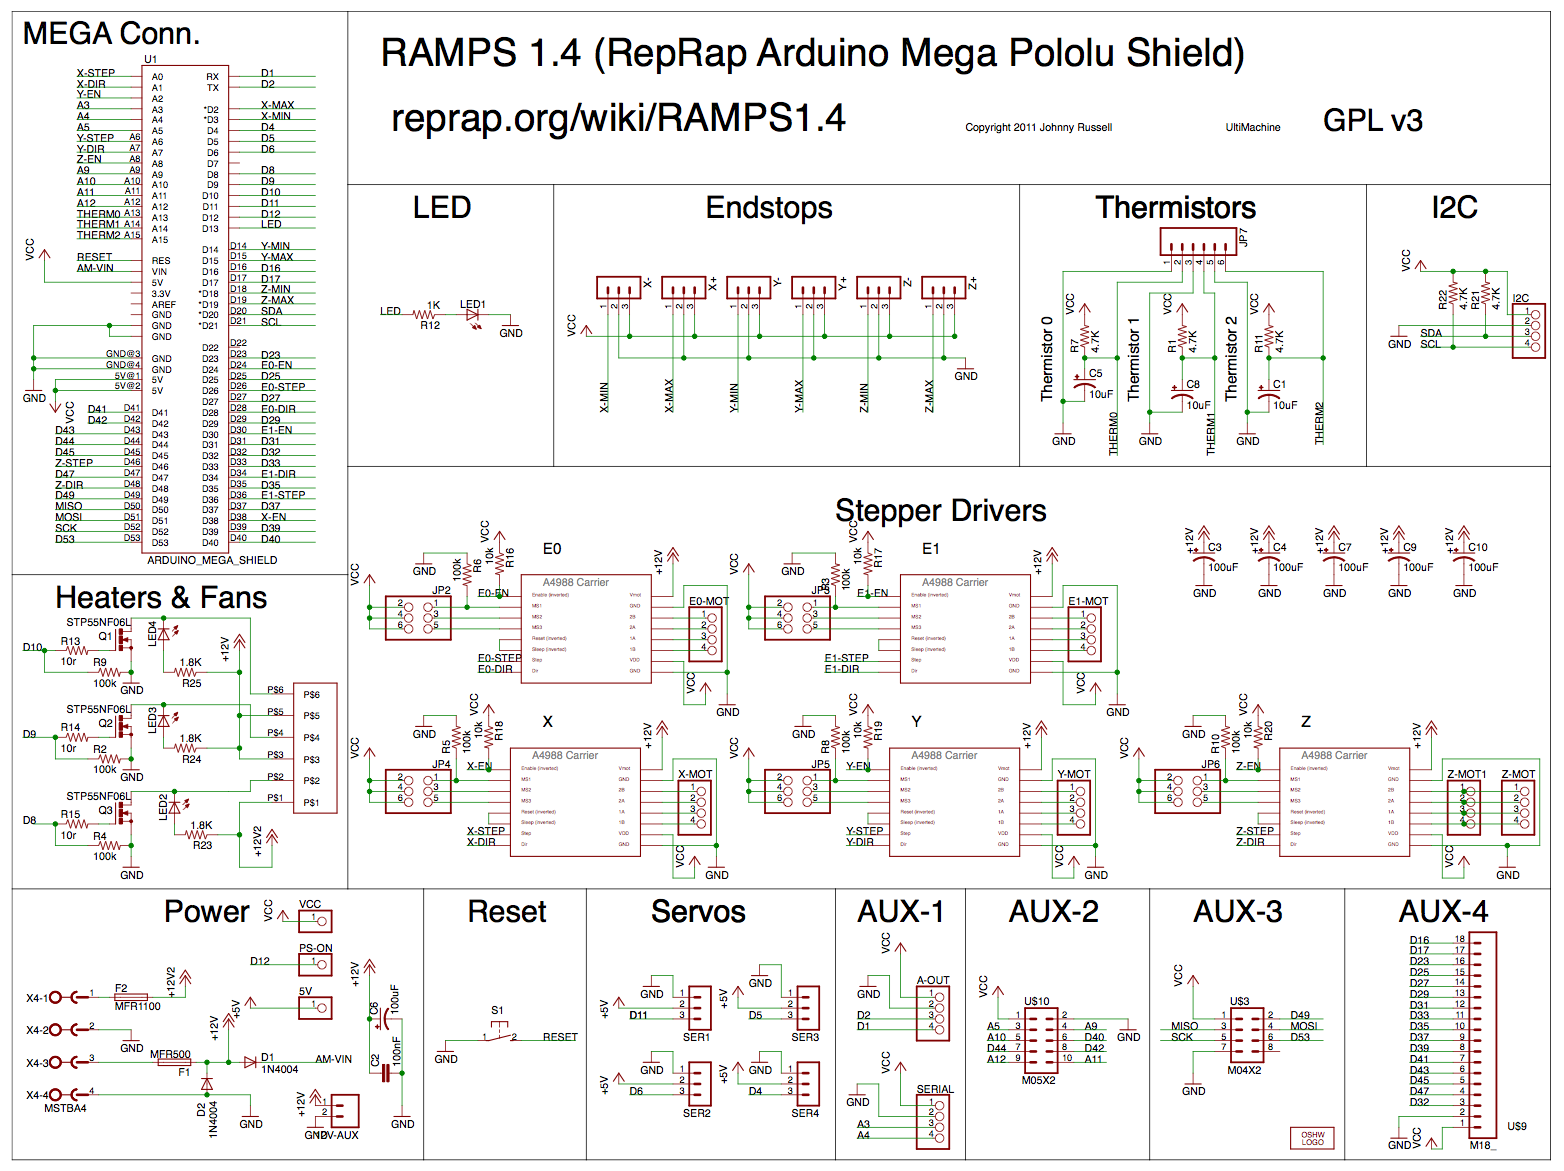
\includegraphics[width=1.0\textwidth, trim = 0px 0px 0px 0px, clip]{./bilder/RAMPS14schematic.png}
  % \end{framed}
  \end{minipage}}
\adjustbox{valign=t}{\begin{minipage}[t]{0.45\textwidth}
% \section{RAMPS 1.4}
\vspace{-4cm}
% \begin{framed}
  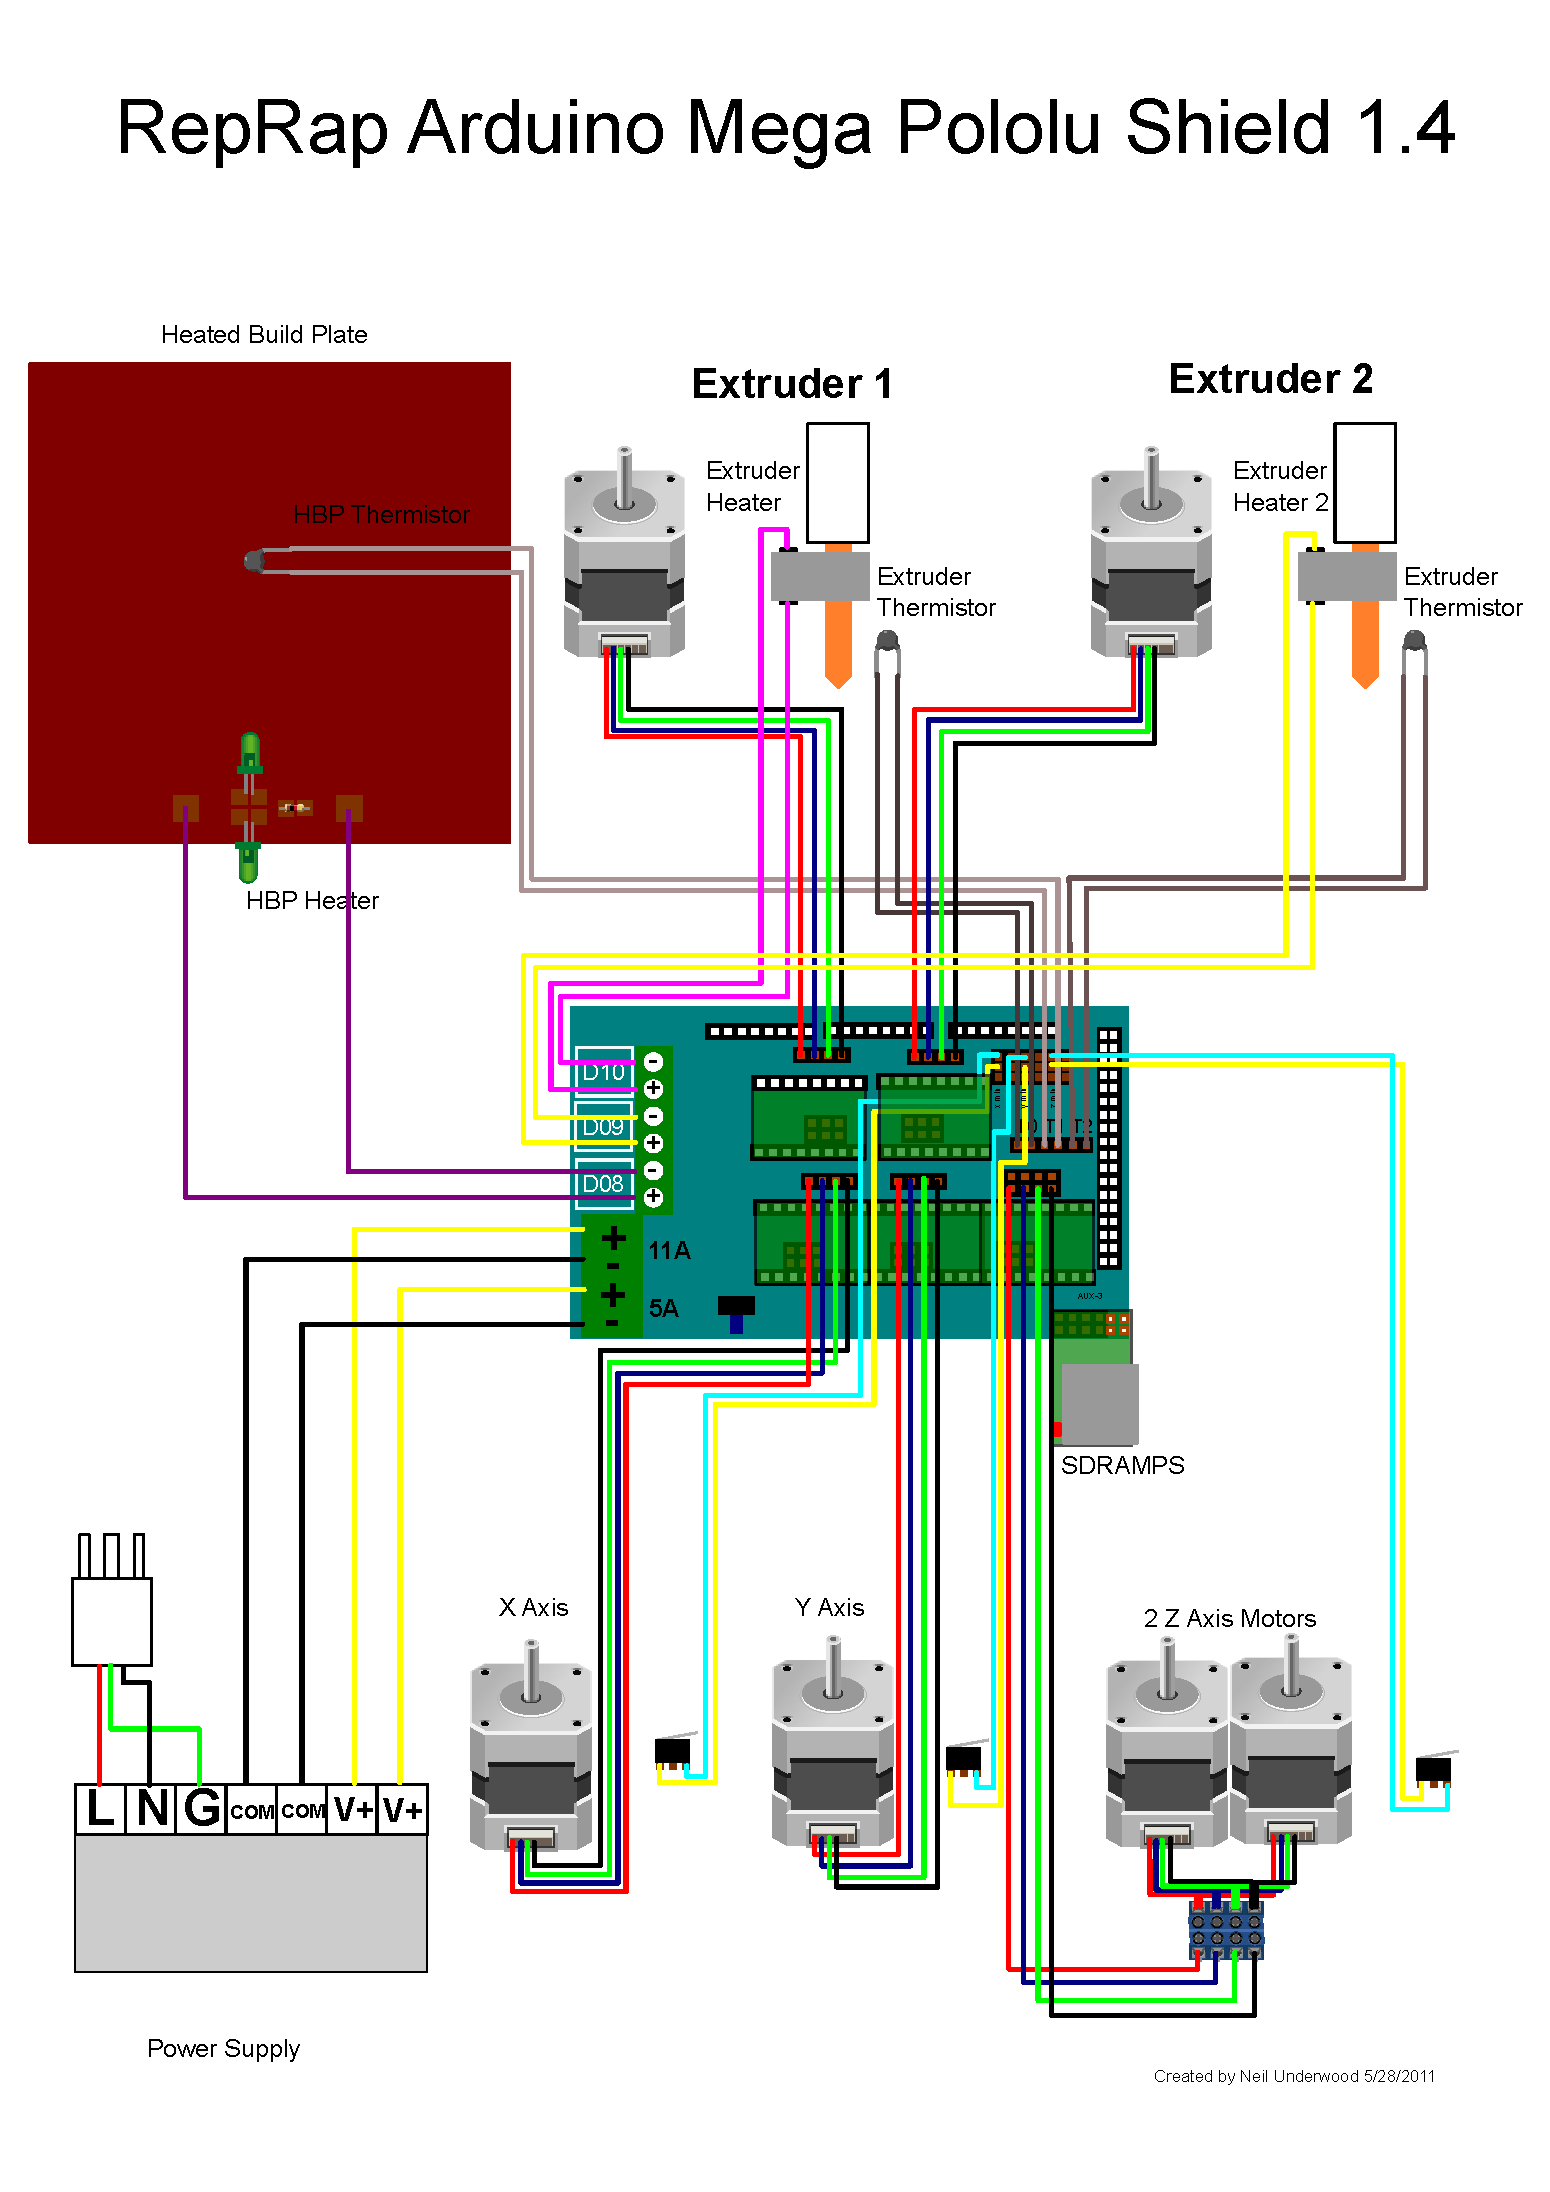
\includegraphics[width=1.0\textwidth, trim = 0px 30px 0px 150px, clip]{./bilder/Rampswire14.pdf}
% \end{framed}
\end{minipage}}
% \hfill
% \hfill
% \end{figure}
% \vspace{0.5cm} % ----------------------------------- vspace
% \begin{figure}[ht]
% \hfill
% ======================================================
\adjustbox{valign=t}{\begin{minipage}[t]{0.45\textwidth}
% \section{SmoothieBoard}
% \vspace{-0.34cm}
% \begin{framed}
  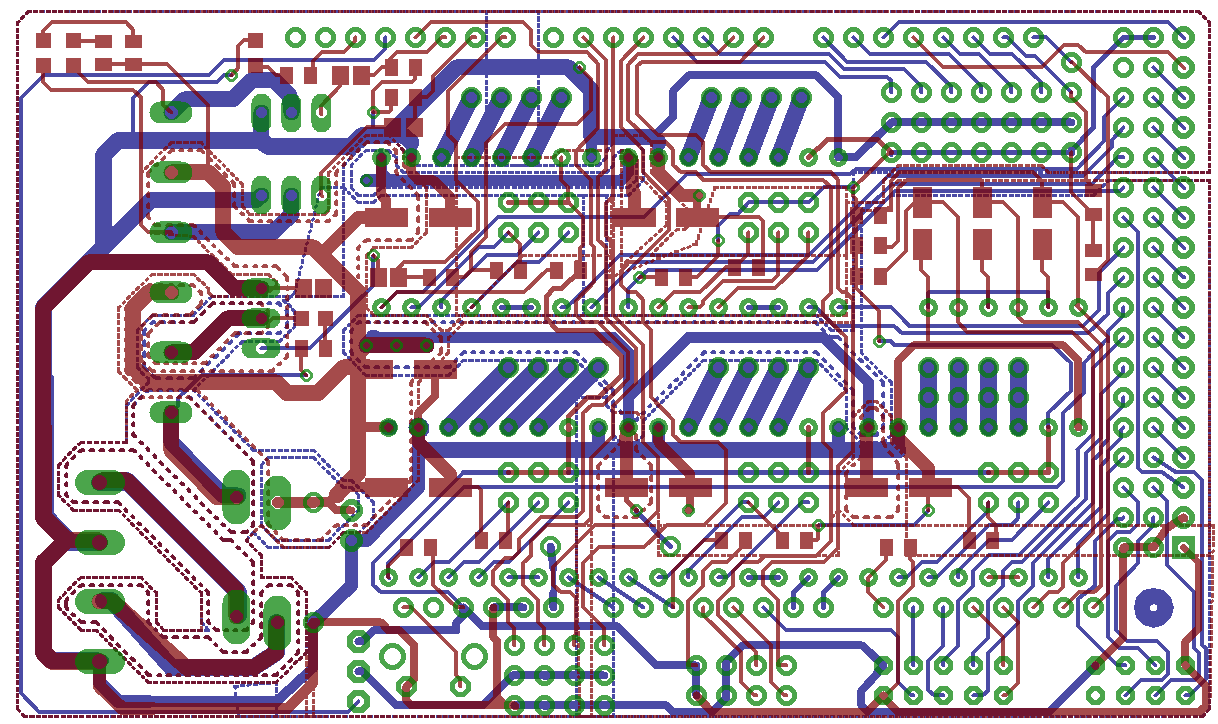
\includegraphics[width=1.0\textwidth, trim = 0px 0px 0px 0px, clip]{./bilder/Ramps14shieldBothsides.png}\\

  Das Smoothieboard ist ähnlich gut Dokumentiert.
% \end{framed}
\end{minipage}}

% ======================================================

% \adjustbox{valign=t}{\begin{minipage}[t]{0.45\textwidth}
% \vspace{0,3cm}
% \huge
% \textbf{Nachteile}
% \begin{itemize}
%   \item 32bit 120 MHz, viel Flash/Ram,
%   \item Lan-Anschluss, 4 Thermal-Sensoren
%   \item Mit Stepper-Driver bestückt
% \end{itemize}
%
% % \caption{Kapazität}
% \end{minipage}}
\end{figure}

\clearpage % GleitObjekte anzeigen

\newpage % ============================================= Newpage ===================
 %  Steuerung
\begin{figure}[ht]
  \section{Heatbed}
\adjustbox{valign=t}{\begin{minipage}[t]{0.30\textwidth}
\begin{framed}
  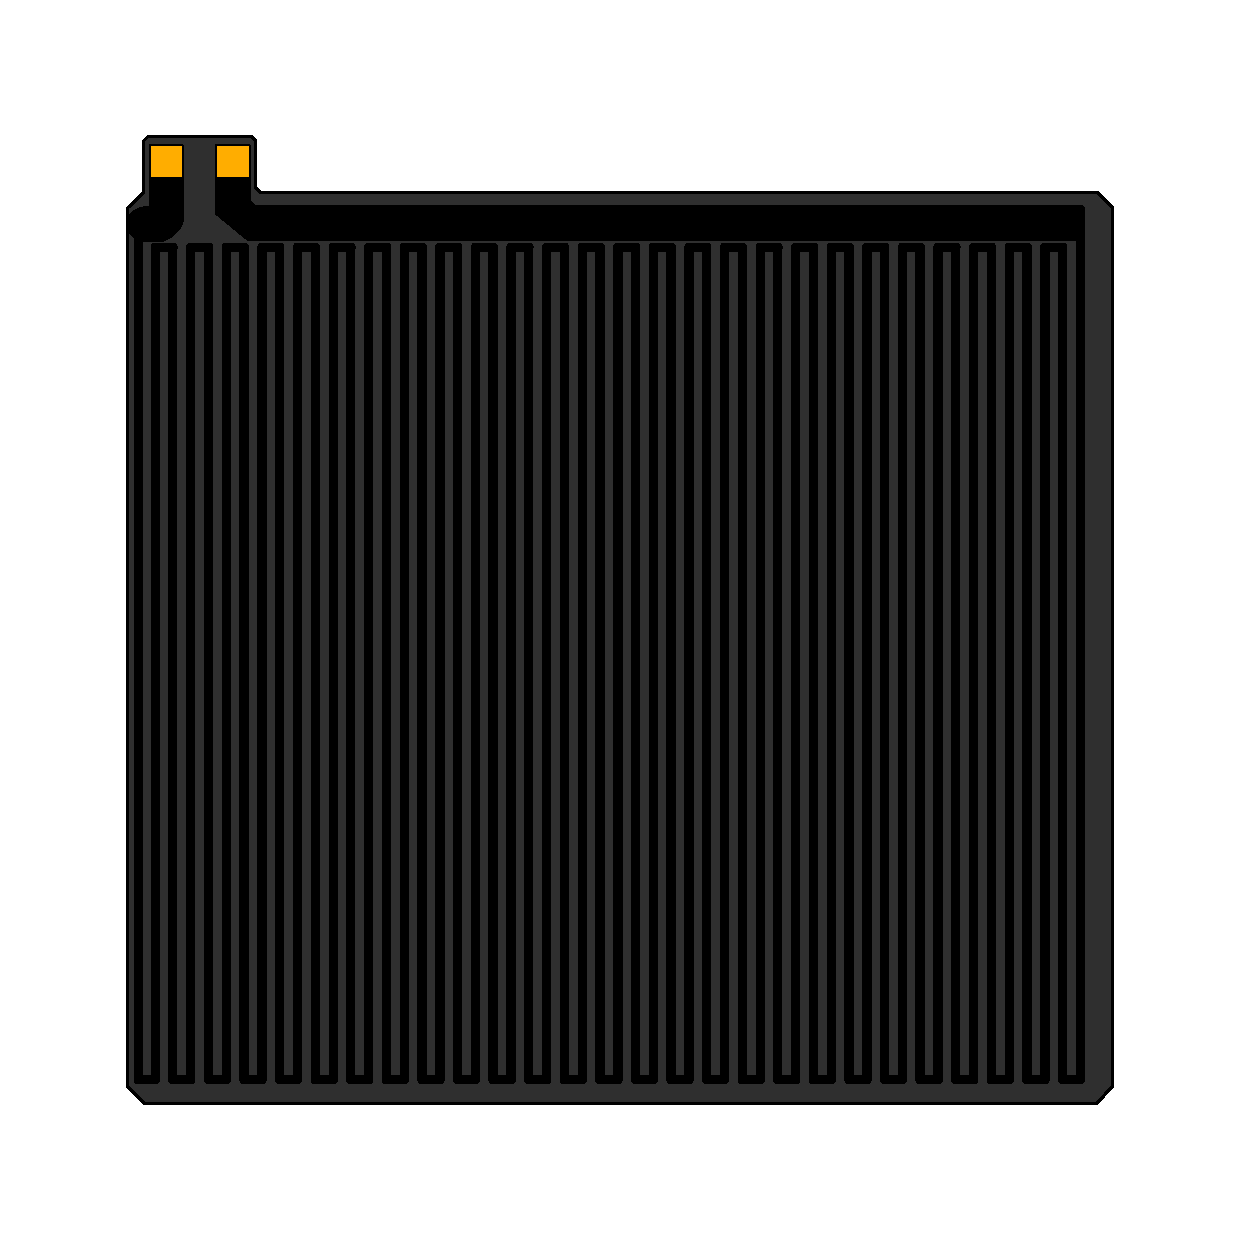
\includegraphics[width=1.0\textwidth, trim = 50px 50px 50px 50px, clip]{./bilder/MK3Bed.pdf}
\end{framed}

\end{minipage}}
% \hfill
\adjustbox{valign=t}{\begin{minipage}[t]{0.60\textwidth}
\vspace{0pt}
\subsection{MK2/MK3 und ähnliche}
\huge
Die meisten PCB / ALU - Heatbed haben eine einzelne Heizschleife. Deshalb konzentriert sich die Wärme in der Mitte und fällt gegen den Rand ab.
% \caption{Kapazität}
\end{minipage}}
% \end{figure}
% \vspace{0.5cm} % ----------------------------------- vspace
% \begin{figure}[ht]
\adjustbox{valign=t}{\begin{minipage}[t]{0.30\textwidth}
% \vspace{0.5cm}
\begin{framed}
  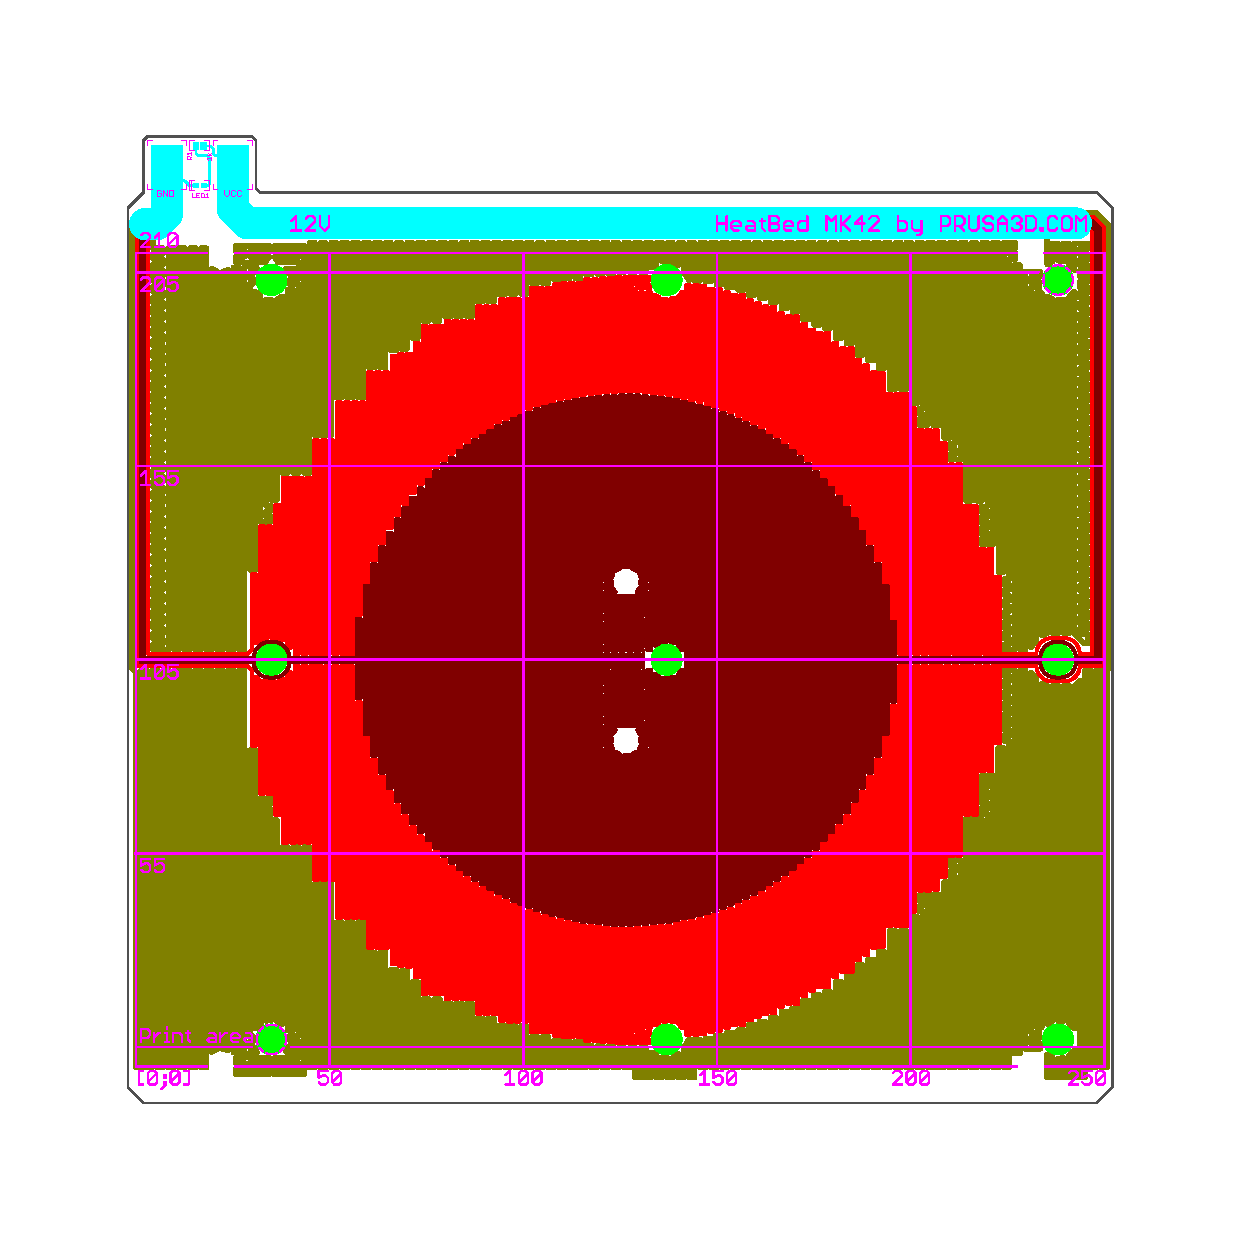
\includegraphics[width=1.0\textwidth, trim = 50px 50px 50px 50px, clip]{./bilder/MK42Bed.pdf}
\end{framed}

\end{minipage}}
\hfill
\adjustbox{valign=t}{\begin{minipage}[t]{0.60\textwidth}
\vspace{0pt}
\subsection{MK42}
\huge
Das MK42 hat 3 verschiedene Heizzonen.\\
Dadurch ist die Oberfläche gleichmäßig beheizt.
Es verfügt über 9 Kalibrierungspunkte welche eine X Y Z Autokalibrierung ermöglichen.
% \caption{Kapazität}
\end{minipage}}
\end{figure}

\clearpage % GleitObjekte anzeigen

\newpage % ============================================= Newpage ===================

\section{Hotend und Extruder}
\begin{center}
  Es gibt 2 Arten von Hotend / Extruder Setups ...
\end{center}

% \begin{framed}

% \end{framed}
\begin{center}
  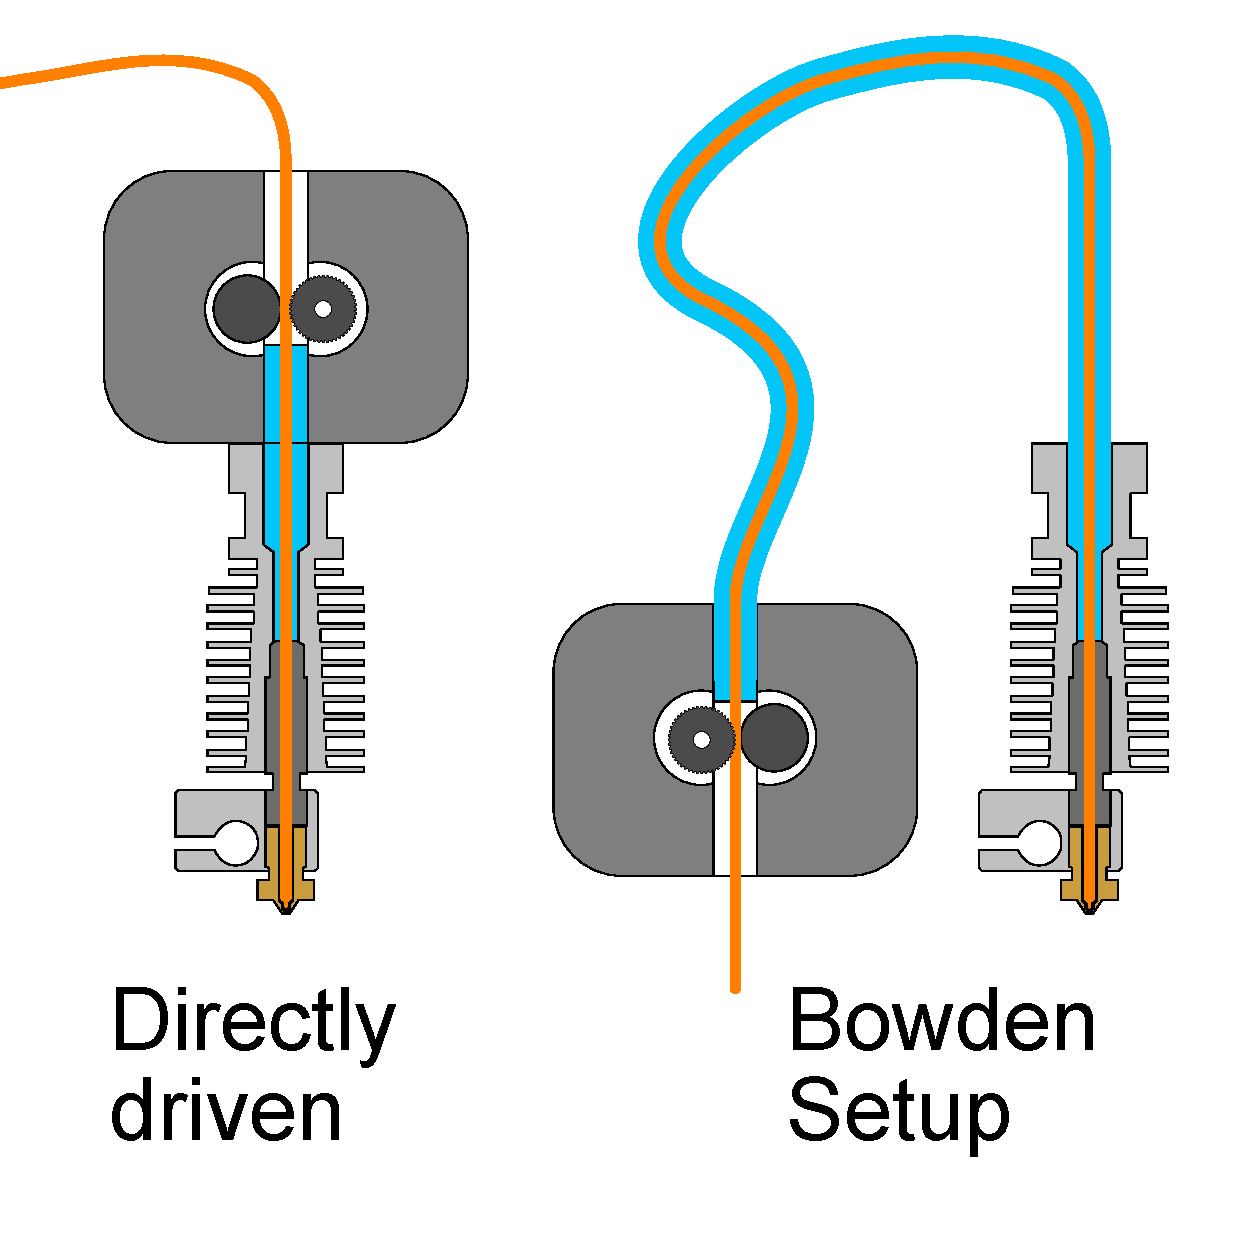
\includegraphics[scale=0.6]{./bilder/Extruder.pdf}
\end{center}

\newpage % ============================================= Newpage ===================

\section{Ein Delta ohne Riemen}
\vspace{1cm}
\begin{center}
  Ein Drucker ohne Zahnriemen in Delta-Bauweise ist sehr gut umsetzbar.
\end{center}
\vspace{1cm}
\begin{itemize}
  \item Es müssen keine Bänder nachgespannt werden
  \item Kein \"{} Spiel \"{} zwischen den Riemen und den Antriebsrädern.
  \item Durch direkten Antrieb und einer Übersetzung ist eine hohe \\ Geschwindigkeit bei gleichzeitig hoher Präzision möglich.
  \item Bei einem Delta spart man generell einen Motor
\end{itemize}

\newpage % ============================================= Newpage ===================

\subsection{Der Drucker in der Ausgangsstellung}
\begin{center}
  Alle Endschalter lösen aus. \\Der Drucker hat den Druckkopf ganz nach oben gefahren.
\end{center}

% \begin{framed}

% \end{framed}
\begin{center}
  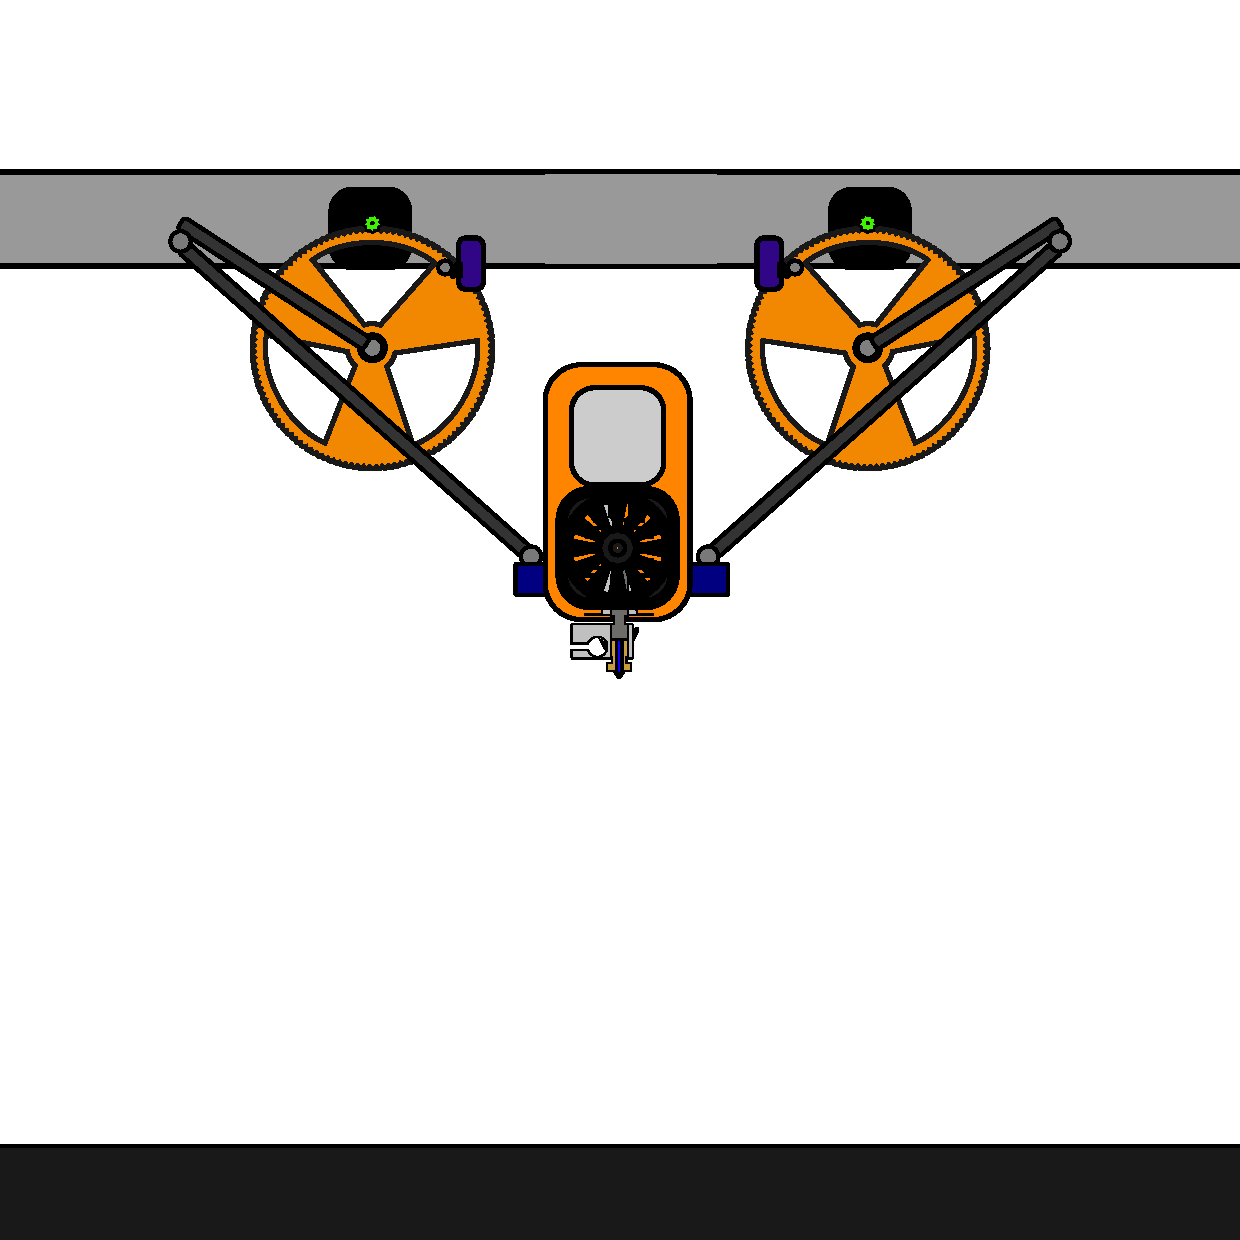
\includegraphics[scale=0.5]{./bilder/mydelta.pdf}
\end{center}

\newpage % ============================================= Newpage ===================

\subsection{Drucker mit abgesenktem Hotend}
% \begin{center}
%   Es gibt 2 Arten von Hotend / Extruder Setups ...
% \end{center}

% \begin{framed}

% \end{framed}
\begin{center}
  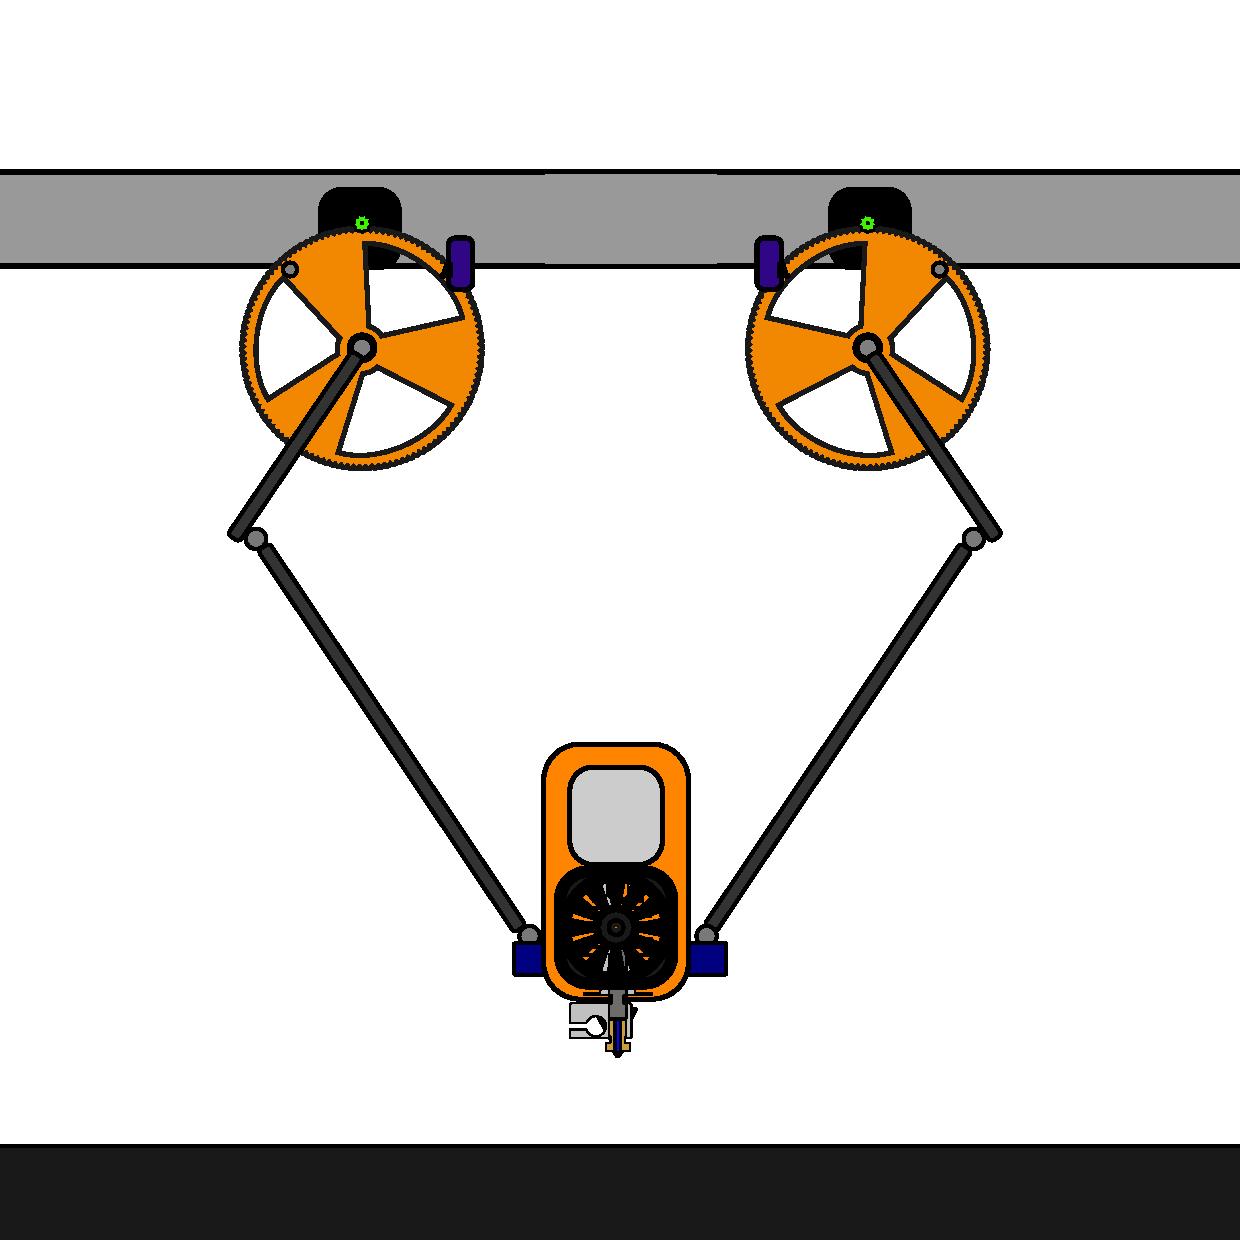
\includegraphics[scale=0.6]{./bilder/mydeltaDown.pdf}
\end{center}

\newpage % ============================================= Newpage ===================

\subsection{Drucker mit nach links gefahrenen Druckkopf }
% \begin{center}
%   Es gibt 2 Arten von Hotend / Extruder Setups ...
% \end{center}

% \begin{framed}

% \end{framed}
\begin{center}
  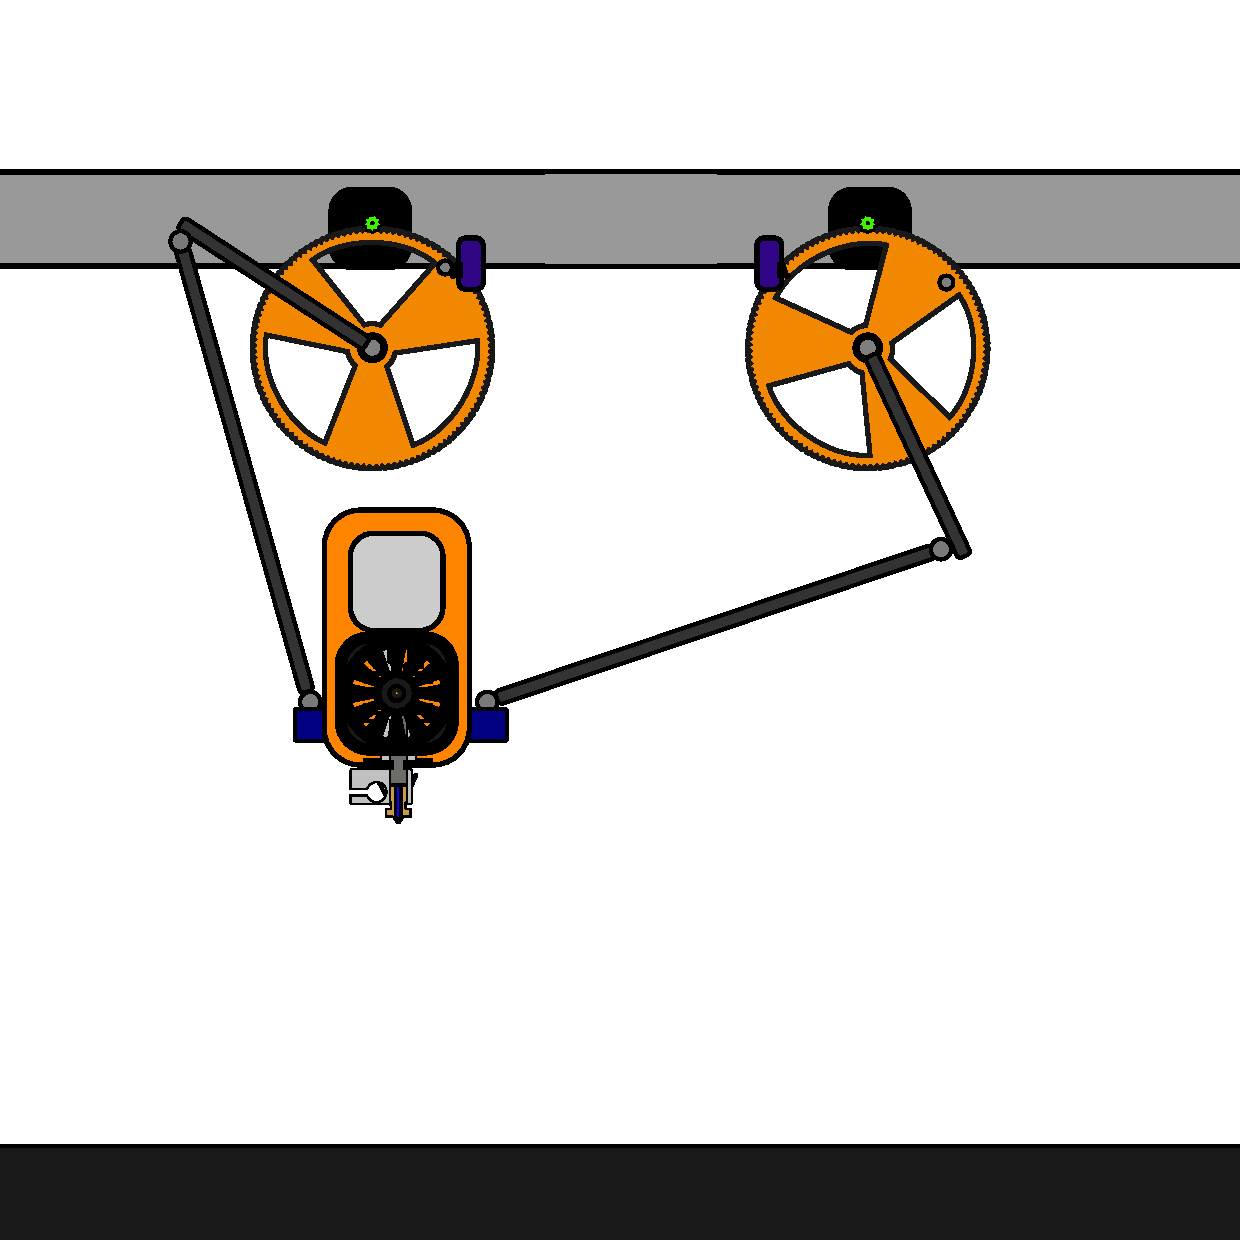
\includegraphics[scale=0.6]{./bilder/mydeltaleft.pdf}
\end{center}
 % Heatbed

% \input{dummy.tex}
% \input{dummy.tex}
% \input{dummy.tex}
% \input{dummy.tex}

% \input{prog1.tex}



%  die beiden unteren beiden includen

% \input{kap1_vorl.tex}
% \input{kap2_vorl.tex}
% \input{kap3_vorl.tex}
% \input{kap4_vorl.tex}
% \input{kap5_vorl.tex}
% \input{kap6_vorl.tex}
% kapitel 7 im Buch

%   Kapitel 2

% \input{2ndKap7.tex}




%==============================================

% % programmieren 2

% \input{kap8.tex}
% \input{kap9.tex}
% \input{kap10.tex}
% \input{kap11.tex}
% \input{kap12.tex}
% \input{last.tex}
% \input{einfuerung.tex}




%=========================================================================================================================
%
%-------------END
\end{document}
